%%
%%  AaltoTheses - LaTeX-tutkielmapohjat Aalto-tyylille
%%
%%  Hannu Tiitu
%%  hannu@tiitu.fi
%%
\begin{filecontents*}{\jobname.xmpdata}
  \Title{Feasibility of profitable betting on FIFA World Cup tournaments}
  \Author{Ville Toiviainen}
  \Keywords{football prediction\sep random forest\sep Kelly's criterion \sep classification\sep recursive feature elimination\sep betting}
  \Publisher{Aalto University}
\end{filecontents*}
\documentclass[oneside,pdfa]{aaltoseries}
\makeatletter
\@ifpackageloaded{inputenc}{%
  \inputencoding{utf8}}{%
  \usepackage[utf8]{inputenc}}
\hypersetup{hidelinks}                % Linkkien korostus pois
\makeatother
\usepackage[finnish,english]{babel}   % Kieli on englanti, tiivistelmässä suomi
\usepackage{setspace}                 % Rivivälin säätämiseksi
\usepackage{afterpage}                % Sivun taustaväri
\microtypesetup{letterspace=25}       % Kannen harvaan välistykseen
\usepackage{dcolumn}
\usepackage{amsmath}
\usepackage{float}
\usepackage[ruled,vlined]{algorithm2e}
\usepackage{bm}
\usepackage{rotating}
\usepackage{booktabs}
\usepackage{array}
\newcolumntype{L}{>{\arraybackslash}m{10cm}}



\author{Ville Toiviainen}
\title{Feasibility of profitable betting on FIFA World Cup tournaments}

\begin{document}



%%  KANSI  ---------------------------------------------

\thispagestyle{empty}
\setcounter{page}{0}  % Kansisivulle sivunumero 0

% Kansisivun marginaalit
\newgeometry{left=23.2mm,right=23.2mm,top=13.5mm,bottom=18mm}

% Musta kansisivu
\pagecolor{aaltoBlack}\afterpage{\nopagecolor}
{\color{white}  % Valkoinen teksti alkaa

{\parindent0pt % Kappaleiden sisennys pois päältä
{\fontsize{11.9pt}{11.9pt}\bfseries\sffamily\lsstyle Master’s Programme in Computer, Communication and Information Sciences}

\vspace{13.1mm}

\begin{spacing}{3.1}
{\fontsize{35}{35}\selectfont Feasibility of profitable betting on FIFA World Cup tournaments}
\end{spacing}

\vspace{7.2mm}

\rule{\textwidth}{1.25pt}

\vspace{8.5mm}

{\fontsize{13.9pt}{13.9pt}\bfseries\sffamily\lsstyle Ville Toiviainen}

\vfill

\begin{picture}(0,0)
\put(356,-7.8){\bfseries\sffamily\footnotesize\lsstyle MASTER'S}
\put(356,-17.4){\bfseries\sffamily\footnotesize\lsstyle THESIS}
\put(346,-26.5){\rule{.75pt}{25pt}}
\end{picture}

\AaltoLogoSmall{.66}{?}{white}

} % Kappaleiden sisennys takaisin käyttöön
} % Valkoisen tekstin pääätös



%%  NIMIÖSIVU  -----------------------------------------

\newpage

\pagenumbering{roman}

% Nimiösivun marginaalit
\newgeometry{left=80.7mm,right=25mm,top=12.9mm,bottom=21mm}

\thispagestyle{empty}

{\parindent0pt % Kappaleiden sisennys pois päältä
\begin{spacing}{1.1}
\hspace{-39.1mm}{\fontsize{10.5pt}{10.5pt}\sffamily\lsstyle Aalto University}

\hspace{-39.1mm}{\fontsize{10.5pt}{10.5pt}\bfseries\sffamily\lsstyle MASTER'S THESIS} {\sffamily\lsstyle 2017}
\end{spacing}

\vspace{12.7mm}

\begin{spacing}{1.63}
{\fontsize{17.8pt}{17.8pt}\selectfont Feasibility of profitable betting on FIFA World Cup tournaments}
\end{spacing}

\vspace{10.6mm}

{\fontsize{13.9pt}{13.9pt}\bfseries\sffamily\lsstyle Ville Toiviainen}

\vfill

{\fontsize{10.3pt}{10.3pt}\sffamily\lsstyle\raggedright
\begin{spacing}{1.06}

Thesis submitted in partial fulfillment of the requirements for the
degree of Master of Science in Technology.

Otaniemi, 19 Nov 2018

\begin{tabbing}
Supervisor:\hspace{6mm} \= professor Aristides Gionis \\
\end{tabbing}
\vspace{-4mm}
\end{spacing}
} % fontsize

\vspace{11.5mm}

\begin{spacing}{.9}
{\bfseries\sffamily\lsstyle Aalto University \\
School of Science \\
Master’s Programme in Computer, Communication and \\Information Sciences}
\end{spacing}
} % Kappaleiden sisennys takaisin käyttöön



%%  ABSTRACT  ------------------------------------------

\newpage
\phantomsection
\addcontentsline{toc}{chapter}{Abstract}

% Tiivistelmien marginaalit
\newgeometry{left=41.8mm,right=25mm,top=14.33mm,bottom=27mm}
% Alkuperäisessä Aalto-sarjassa marginaalit ovat suunnilleen näin:
%\newgeometry{left=41.8mm,right=17.6mm,top=14.33mm,bottom=20.4mm}

\begin{spacing}{.88}

{\parindent0pt % Kappaleiden sisennys pois päältä
\AaltoLogoSmall{.625}{''}{aaltoBlack}

{\fontsize{13.9pt}{13.9pt}\selectfont
\vspace{-8.9mm}\hfill{\bfseries\sffamily\lsstyle Abstract}}

{\fontsize{9.48pt}{9.48pt}\selectfont
\vspace{.9mm}\hfill{\bfseries\sffamily\lsstyle Aalto University, P.O. Box 11000, FI-00076 Aalto~~\textcolor{aaltoGray}{www.aalto.fi}}}

\vspace{7.8mm}{\fontsize{10.5pt}{10.5pt}\bfseries\sffamily\lsstyle Author}\\
{\small Ville Toiviainen}

\vspace{-2.4mm}\rule{\textwidth}{.75pt}

{\fontsize{10.5pt}{10.5pt}\bfseries\sffamily\lsstyle Title}\\
\parbox[t]{\textwidth}{\raggedright\small Feasibility of profitable betting on FIFA World Cup tournaments}

\vspace{.5mm}\rule{\textwidth}{.75pt}

{\fontsize{10.5pt}{10.5pt}\bfseries\sffamily\lsstyle School}~~{\small School of Science}

\vspace{-2.4mm}\rule{\textwidth}{.75pt}

{\fontsize{10.5pt}{10.5pt}\bfseries\sffamily\lsstyle Master's programme}~~{\small Computer, Communication and Information Sciences}

\vspace{-2.4mm}\rule{\textwidth}{.75pt}

{\fontsize{10.5pt}{10.5pt}\bfseries\sffamily\lsstyle Major}~~{\small  Machine Learning and Data Mining}\hfill{\fontsize{10.5pt}{10.5pt}\bfseries\sffamily\lsstyle Code}~~{\small SCI3044}

\vspace{-2.4mm}\rule{\textwidth}{.75pt}

{\fontsize{10.5pt}{10.5pt}\bfseries\sffamily\lsstyle Supervisor}~~{\small professor Aristides Gionis}

\vspace{-2.4mm}\rule{\textwidth}{.75pt}

{\fontsize{10.5pt}{10.5pt}\bfseries\sffamily\lsstyle Level}~~{\small Master's thesis}\hfill{\fontsize{10.5pt}{10.5pt}\bfseries\sffamily\lsstyle Date}~~{\small 19 Nov 2018}\hfill{\fontsize{10.5pt}{10.5pt}\bfseries\sffamily\lsstyle Pages}~~{\small 46}\hfill{\fontsize{10.5pt}{10.5pt}\bfseries\sffamily\lsstyle Language}~~{\small English}

\vspace{-2.4mm}\rule{\textwidth}{.75pt}

\vspace{6mm}

} % Kappaleiden sisennys takaisin käyttöön
\end{spacing}
\begin{spacing}{1.05}

\noindent{\fontsize{10.5pt}{10.5pt}\bfseries\sffamily\lsstyle Abstract}
\vspace{.8mm}

{\small
  This thesis examines the feasibility of building a profitable betting system that bets on FIFA World Cups. Existing literature has researched the opportunity to bet on football games, but not in the context of FIFA World Cups. Most of the existing literature related to FIFA World Cups has examined how to predict the most probable winner or what the most probable course of the tournament might be.

  In this thesis, tournaments are predicted using tree-based models and a linear model. All of the models are trained using a dataset on historical matches and a player attribute dataset obtained from the EA Sport's video game series FIFA. A more in-depth analysis of the engineered features is performed using different combinations of the features and with recursive feature elimination process. Models' output is used with a betting strategy based on Kelly's criterion and with a betting strategy that places one unit for the most probable winner.

  Two of the models are profitable in all of the tested tournaments, and most of the models can be profitable at least in two out of the three tested tournaments. However, guaranteed profits cannot be stated with full confidence since the number of games in total is relatively small. Data limitations limit the possibility to test the model with more tournaments. Using video game data with historical matches increased the accuracy in probability predictions. Models predict the probability of a home win and an away win very similarly, but predict the probability of a draw differently. Models do not prefer a draw as the most probable outcome in almost all of the matches.
}

\vfill

\end{spacing}
\begin{spacing}{.88}
{\parindent0pt % Kappaleiden sisennys pois päältä

\makebox[19mm][l]{\fontsize{10.5pt}{10.5pt}\bfseries\sffamily\lsstyle Keywords}\parbox[t]{123.6mm}{\raggedright\small football prediction, random forest, Kelly's criterion  classification, recursive feature elimination, betting}

\vspace{.5mm}\rule{\textwidth}{.75pt}

{\fontsize{10.5pt}{10.5pt}\bfseries\sffamily\lsstyle urn}~~{\small http://urn.fi/URN:NBN:fi:aalto-201712188201}

\vspace{-2.4mm}\rule{\textwidth}{.75pt}

} % Kappaleiden sisennys takaisin käyttöön
\end{spacing}



%%  TIIVISTELMÄ  ---------------------------------------

\newpage
\phantomsection
\addcontentsline{toc}{chapter}{Tiivistelmä}

% Tiivistelmäsivu suomeksi
\selectlanguage{finnish}

\begin{spacing}{.88}

{\parindent0pt % Kappaleiden sisennys pois päältä
\AaltoLogoSmall{.625}{!}{aaltoBlack}

{\fontsize{13.9pt}{13.9pt}\selectfont
\vspace{-8.9mm}\hfill{\bfseries\sffamily\lsstyle Tiivistelmä}}

{\fontsize{9.48pt}{9.48pt}\selectfont
\vspace{.9mm}\hfill{\bfseries\sffamily\lsstyle Aalto-yliopisto, PL 11000, 00076 Aalto~~\textcolor{aaltoGray}{www.aalto.fi}}}

\vspace{7.8mm}{\fontsize{10.5pt}{10.5pt}\bfseries\sffamily\lsstyle Tekijä}\\
{\small Ville Toiviainen}

\vspace{-2.4mm}\rule{\textwidth}{.75pt}

{\fontsize{10.5pt}{10.5pt}\bfseries\sffamily\lsstyle Työn nimi}\\
\parbox[t]{\textwidth}{\raggedright\small Feasibility of profitable betting on FIFA World Cup tournaments}

\vspace{.5mm}\rule{\textwidth}{.75pt}

{\fontsize{10.5pt}{10.5pt}\bfseries\sffamily\lsstyle Korkeakoulu}~~{\small Perustieteiden korkeakoulu}

\vspace{-2.4mm}\rule{\textwidth}{.75pt}

{\fontsize{10.5pt}{10.5pt}\bfseries\sffamily\lsstyle Maisteriohjelma}~~{\small Computer, Communication and Information Sciences}

\vspace{-2.4mm}\rule{\textwidth}{.75pt}

{\fontsize{10.5pt}{10.5pt}\bfseries\sffamily\lsstyle Pääaine}~~{\small  Machine Learning and Data Mining}\hfill{\fontsize{10.5pt}{10.5pt}\bfseries\sffamily\lsstyle Koodi}~~{\small SCI3044}

\vspace{-2.4mm}\rule{\textwidth}{.75pt}

{\fontsize{10.5pt}{10.5pt}\bfseries\sffamily\lsstyle Valvoja}~~{\small professori Aristides Gionis}

\vspace{-2.4mm}\rule{\textwidth}{.75pt}

\vspace{-2.4mm}\rule{\textwidth}{.75pt}

{\fontsize{10.5pt}{10.5pt}\bfseries\sffamily\lsstyle Työn laji}~~{\small Diplomityö}\hfill{\fontsize{10.5pt}{10.5pt}\bfseries\sffamily\lsstyle Päiväys}~~{\small 19.11.2018}\hfill{\fontsize{10.5pt}{10.5pt}\bfseries\sffamily\lsstyle Sivuja}~~{\small 46}\hfill{\fontsize{10.5pt}{10.5pt}\bfseries\sffamily\lsstyle Kieli}~~{\small englanti}

\vspace{-2.4mm}\rule{\textwidth}{.75pt}

\vspace{6mm}

} % Kappaleiden sisennys takaisin käyttöön
\end{spacing}
\begin{spacing}{1.05}

\noindent{\fontsize{10.5pt}{10.5pt}\bfseries\sffamily\lsstyle Tiivistelmä}
\vspace{.8mm}

{\small
  Tämä diplomityö tutkii, onko mahdollista toteuttaa voittoatekevä vedonlyöntijärjestelmä jalkapallon maailmanmestaruuskilpailuja varten. Mahdollisuutta tienata vedonlyönnillä jalkapallossa on aiemmin tutkittu. Tämä tutkimus ei ole kuitenkaan ulottunut koskemaan vedonlyöntiä jalkapallon maailmanmestaruuskisoissa. Jalkapallon maailmanmestaruuskisoja koskeva aikaisempi tutkimus on keskittynyt ennustamaan potentiaalista voittajaa tai simuloimaan kuinka kisoissa todennäköisesti käy.

  Tässä diplomityössä jalkapallon maailmanmestaruuskisoja ennustetaan puupohjaisilla malleilla ja lineaarisella mallilla. Kaikki käytetyt mallit koulutetaan syötteellä, joka on generoitu kahdesta eri datalähteestä: historiallisista otteludatasta sekä videopelin “EA Sport’s video game series FIFA” pelaaja-attribuuttidatasta. Syötteen merkittävyyttä tutkitaan tarkemmin hyödyntäen erilaisia syötekombinaatioita sekä toteuttamalla rekursiivinen syötteen eliminointiprosessi. Mallien tulostetta käytetään kahdessa vedonlyöntistrategiassa. Ensimmäinen strategia lyö vetoa voittajan puolesta ja toinen strategia hyödyntää Kellyn kriteeriä vedonlyöntikohteiden valinnassa.

  Kaksi mallia on voitollisia kaikissa kokeiluissa turnauksissa ja suurin osa malleista on voitollisia ainakin kahdessa kokeiluista turnauksista. Tuloksien luotettavuutta heikentää rajattu turnauksien määrä mitä testauksessa voidaan käyttää. Videopeleissä käytetyn datan hyödyntäminen ennustamisessa osoittautui hyödylliseksi. Kaikki mallit ennustavat koti- ja vierasjoukkueen voiton hyvin samankaltaisesti. Eniten eroavaisuuksia mallien välillä on tasapelin ennustamisessa. Mallit eivät pidä kovinkaan usein tasapelia kaikista todennäköisempänä lopputuloksena.
}

\vfill

\end{spacing}
\begin{spacing}{.88}
{\parindent0pt % Kappaleiden sisennys pois päältä

\makebox[21mm][l]{\fontsize{10.5pt}{10.5pt}\bfseries\sffamily\lsstyle Avainsanat}\parbox[t]{121.6mm}{\raggedright\small football prediction, random forest, Kelly's criterion  classification, recursive feature elimination, betting}

\vspace{.5mm}\rule{\textwidth}{.75pt}

{\fontsize{10.5pt}{10.5pt}\bfseries\sffamily\lsstyle urn}~~{\small http://urn.fi/URN:NBN:fi:aalto-201712188201}

\vspace{-2.4mm}\rule{\textwidth}{.75pt}

} % Kappaleiden sisennys takaisin käyttöön
\end{spacing}

\selectlanguage{english}  % Palataan englantiin
\restoregeometry  % Palataan normaaleihin sivumarginaaleihin



%%  SISÄLTÖ  -------------------------------------------

\newpage

\tableofcontents

%%  TYÖ ALKAA TÄSTÄ  -----------------------------------

\newpage

\pagenumbering{arabic}

\chapter{Introduction}
Main motivation behind this master's thesis is to experiment how accurately an outcome of a football match in a World cup tournament can be predicted and is it possible to create a profitable betting strategy for the tournament. To "beat the bookie" only freely accessible data can be used.

Football, being one of the biggest sports in the world, attracts lot of global attention especially during the main tournaments like FIFA World Cup and EURO. This global interest has attracted big investment banks like Goldman Sachs and UBS to predict tournament outcome. Also, the research community has been active around this topic; mostly predicting the probabilities for winning the tournament or predicting the most probable course of the tournament \cite{groll2018prediction, groll2015prediction, leitner2010forecasting}.

For many betting the outcome of a match is as important part of the experience as watching the game. No wonder that the size of the betting industry is massive. This must be one the reason why the field of economics has actively research this industry, especially the efficiency of the betting market. When markets are efficient all the available information is reflect in the prices and there is no change to "beat the market". This efficient market hypothesis of betting market has been discarded by \cite{vlastakis2009efficient} - even the weak-form of efficient market hypothesis. Even though the betting markets are not efficient the general assumption is that probabilities given by the betting industry are close to the true probabilities. For this reason models are often benchmarked against the odds given by the betting industry and can be useful features as well. \cite{leitner2010forecasting}. Kuypers \cite{kuypers2008} has heavily claims against the believe that the betting market consensus is close to the true probabilities. If bookmaker wants to increase its profits while keeping its over-roundness competitive it needs set the odds further from the market efficient odds. Also, marketing purposes and heavy one-sided bets can lead to inefficient odds. In the case of heavy one-sided bets bookmaker exposes itself to a higher risk exposure if the match's outcome is the one that is betted very heavily. Major tournaments like FIFA World Cup increase the betting activity. The hypothesis is that this can lead to odds that are further away from the true probabilities which naturally leads to a question: is it possible to earn profit from betting FIFA World Cup matches?

As far as I know this opportunity to bet profitably on FIFA World Cup has not been researched. For this reason one of the main goals of this master's thesis is to investigate if it's possible to create a profitable betting strategy for FIFA World Cup.

Nowadays, data is collected extensively from different sports. For long data collection in football was limited compared to other sports like basketball, but now many different sources for data exists. Unfortunate part is, that the data is very expensive and only part of it is freely available. Free data mostly contains historical matches. Fortunately many games that simulate football have a vast collection of player and team-level attribute data. This data is freely available and to my knowledge has been successfully used once \cite{shin2014novel}. Can this freely available data on players and historical matches be used to predict the tournaments more accurately than the betting market predicts?

This thesis will answer to these two questions: "Is it possible to bet FIFA World Cup matches profitably?" and "Is it possible to predict the tournaments more accurately than the betting market predicts?". The idea is not to seek for abnormal odds, but to use the average odds from the markets wisely. If positive profits exist in this scenario, "beating the bookie" is not impossible.

The rest of the thesis is structured as follows: in Literature review I go through the existing research on the topic. Next in Section 3 I describe the dataset and how player attributes are aggregated to team-level attributes. Then, in Section 4, I describe the prediction models, betting strategies and the tournament simulation process. In Section 5 results from the simulation experiments are stated. Finally I conclude and discuss about future work in Section 6.

\chapter{Literature Review}
Modeling football scores has gained some interest in scientific communities. One of the first to mention that football score distribution resemble a Poisson distribution was Maronoey \cite{moroney1962facts} in his book Facts from figures. Although Poisson distributed fitted the scores well he came into a conclusion that using the negative binomial distribution could be an improvement.
In 1997 Dixon stated \cite{dixon1997} "It's not difficult to predict fairly accurately which teams are likely to be successful, but the development of models that have a sufficiently high resolution to exploit this long run predictive capability for individual matches is substantially more difficult." Chance dominates the game. However Maher \cite{maher1982modelling} idea to  included team's quality into the model was promising. He used independent Poisson distribution is his model to model the score based on team's previous performance. Over ten years later Dixon used a similar approach in his model and was able to achieve positive returns from betting \cite{dixon1997}.

The key with these kind of models is to describe the team's quality as well as possible. Elo rating, originally developed for assessing the strength of chess players \cite{elo1978rating}, has gained popularity in football prediction. Leitner et al. \cite{leitner2010forecasting} simulated UEFA Euro 2008 football tournament using ratings of abilities (such as the Elo rating or FIFA/Coca-Cola World ranking) and Bookmaker's odds. They showed that Bookmarker's odds outperformed Elo and FIFA/Coca-Cola World ranking, but both are suitable attributes for match outcome prediction. When ratings of abilities were compared FIFA/Coca-Cola World \footnote{FIFA has changed the ranking algorithm three times since it was introduced. The ranking algorithm will be changed after FIFA World Cup 2018 to resemble Elo rating \cite{wiki:fifarating}.} rating had a higher Spearman correlation than Elo rating which mean that it would be a better metric if the corresponding winning probabilities could be computed \cite{leitner2010forecasting}. Lasek et al. \cite{lasek2013predictive} results are contrary to these findings. They compared different rating methods and their results imply that Elo rating describes better team's ability compared to FIFA/Coca-Cola rating. Hvattum et al. \cite{hvattum2010using} concluded that the single rating difference is a highly significant predictor of match outcomes which justifies the increasing interest in using Elo rating to describe team's ability. In their study they used logistic regression, but were not able to achieve as good results with using Elo rating only as they were with market odds. More data is needed with Elo rating to match the market's accuracy.

When the number of used features has grown tree based models have gained popularity in football prediction. Groll et al. \cite{groll2018prediction} predicted the FIFA World Cup 2018 match outcomes using three different models: a random forest model, a regression model and a ranking model. From these models the random forest model performed the best in classification and outperformed the bookmakers. For features they used economic factors such as GDP per capita, sportative factors like FIFA/Coca-Cola rating, factors that described the team's structure like average age and factors that described team's coach. A random forest model also outperformed a support vector machine model and a bagging REP tree model in prediction accuracy when the task was to predict the outcome of a match in Turkish super league. In this study feature set selection was performed and a limited feature set performed better than the full feature set. \cite{10.1007/978-3-319-29504-6_48}

One clear motivation behind match outcome prediction is the possibility to earn money from betting. The \textit{Efficient market hypothesis} (EMH) defined by Badarinathi and Kochmann \cite{badarinathi1996football} "asserts that investors cannot consistently "beat the market" because stocks reside in perpetual equilibrium" is a known assumption in finance. Since american football betting market resembles Wall Street Pankoff \cite{pankoff1968market} reasoned that american football betting should be EMH as well. He came to conclusion that the systematic market errors are not large enough to be profitable to bettors. Later the efficient market hypothesis has been revoked in finance \cite{jegadeesh1993returns}, and this might be the case in betting as well \cite{goddard2003modelling, badarinathi1996football}. However Goddard et al. \cite{goddard2003modelling} states that there is some evidence that inefficiencies in the bookmakers’ prices have diminished over time. Kuypers \cite{kuypers2008} analysis on how bookmakers calculate their odds supports this claim of inefficiencies in the bookmakers’ prices. If bookmaker wants to increase its profits while keeping its over-roundness competitive it needs set the odds further from the market efficient odds. Also, marketing purposes and heavy one-sided bets can lead to inefficient odds. In the case of heavy one-sided bets bookmaker exposes itself to higher risk exposure if match's outcome is the one that is betted very heavily. With a proper betting strategy and a model that is able to beat bookmakers generating profit from football betting should be possible.

One well-known betting strategy is Kelly's criterion which has been also used outside of sport betting by famous investors like Warren Buffet and Bill Cross \footnote{http://www.financial-math.org/blog/2013/10/two-tales-of-the-kelly-formula/}. This strategy aims to maximize the logarithm of wealth by placing an optimal fraction of the total bankroll for a bet based on the probabilities. MacLean et al. \cite{maclean1992growth} looked at the benefits of using a fraction of the optimal fraction given by Kelly criterion. They concluded that it's a trade off between small decrease in the growth rate against increased change of doubling your fortune before it's halved. This is a crucial finding since World Cup tournaments have very limited number of games and for a strategy to work, it needs to be successful from the very first games onwards.


% \begin{enumerate}
%     \item What methods and how matches are predicted (Win/lose, score)
%     One factor models, Multifactor models, Score vs outcome prediction, data used in multifactor,
%     \item How simulations are done if any
%     \item Elo rating
%     \item beating bookmaker's odds
% \end{enumerate}



% Groll et al. \cite{groll2018prediction} predicted the FIFA World Cup 2018 match outcomes using three different methods. Data used in their experiments was the as in \cite{groll2015prediction}. This dataset has very limited attributes to describe teams playing styles. Team's ability covariate from the rating method is included in the input vector for the final simulations. Team's ability weights team's recent performance more than FIFA/Coca-Cola World ranking . Including this team's ability parameter improved the accuracy significantly for Random Forest. It's important to notice that the input data used in \cite{groll2018prediction} is not updated during the tournament. This means that ranking stays static even though one team might perform well based on the other attributes and survive far in the tournament. This means that the team's ability is not updated to reflect the real ability based on the prediction results.
% Groll et al. \cite{groll2018prediction} predicted the match outcomes using regression, not classification. With regression, the feature vector is conditional on match's teams but predicted scores are drawn from independent Poisson distributions. With ranking methods score is dependent. Dixon and Coles \cite{dixon1997} identified correlation between scores and are one of the many researchers that have relaxed the strong assumption of conditional independence between the scores.

% Leitner et al. \cite{leitner2010forecasting} simulated UEFA Euro 2008 football tournament using ratings of abilities (such as the Elo rating or FIFA/Coca-Cola World ranking) and Bookmaker's odds. They showed that Bookmarker's odds outperformed Elo, but both are suitable attributes for match outcome prediction. Their models predicted only the probability of a win. This limits the model's accuracy in cases where two or more teams share the same number of points in the group stage. The model which based on the bookmaker's odds was able to predict the teams in the final correctly. One interesting finding in \cite{leitner2010forecasting} is that FIFA/Coca-Cola World \footnote{FIFA has changed the ranking algorithm three times since it was introduced. The ranking algorithm will be changed after FIFA World Cup 2018 to resemble Elo rating \cite{wiki:fifarating}.} rating has a higher Spearman correlation than Elo rating and could be a good metric if the corresponding winning probabilities could be computed. Results in paper \cite{lasek2013predictive} are contrary to these findings. Lasek et al. \cite{lasek2013predictive} compared different rating methods and their results imply that Elo rating describes a better team's ability compared to FIFA/Coca-Cola rating.

% Simulations \cite{leitner2010forecasting, groll2018prediction} are done in a manner which takes into account group draws. Their results show that teams with relatively easier opponents in the group stage have higher probabilities to go further in the tournament.

% One clear motivation behind match outcome prediction is the possibility to earn money from betting. The \textit{Efficient market hypothesis} defined by Badarinathi and Kochmann \cite{badarinathi1996football} "asserts that investors cannot consistently "beat the market" because stocks reside in perpetual equilibrium" is an assumption used in finance. Weak-form efficiency means that a part of the odds given by bookmakers are mispriced. The efficient market hypothesis has been revoked in finance \cite{jegadeesh1993returns}. Goddard et al. and Badarinathi et al. \cite{goddard2003modelling, badarinathi1996football} find that this might be the case in also in betting. However Goddard et al. \cite{goddard2003modelling} states that there is some evidence that inefficiencies in the bookmakers’ prices have diminished over time.

% Kuypers \cite{kuypers2008} shares some light on how bookmakers calculate their odds. If bookmaker wants to increase its profits while keeping its over-roundness competitive it needs set the odds futher from the market effiecient odds. Also, marketing purposes and heavy one-sided bets can lead to inefficient odds. In the case of heavy one-sided bets bookmaker exposes itself to higher risk exposure if match's outcome is the one that is betted very heavily.


\chapter{Data}
In this section, we briefly describe the main datasets: the dataset of international football matches and the dataset of player attributes from the EA Sport's video game series FIFA. We have used both of the datasets to generate new data points. This process will be discussed in this chapter.

\section{International football match dataset}
As the primary source of data we have used results from all international football matches from November 11th, 1872 to June 6th, 2018. This dataset is provided by Kaggle \cite{matchdb} and contains match scores, tournament types, dates and more attributes that are not used in this thesis.

We don't use this dataset directly in prediction. Instead, we extract useful features from this data. Generated features from this dataset are named as \textit{general features}.
\renewcommand{\labelitemi}{}
\begin{description}
    \itemsep0em
    \item[Elo rating] describes the team's quality. This metric is calculated based on previous games with the following formula \begin{equation}
        \mathrm { R } _ { \mathrm { n } } = \mathrm { R } _ { \mathrm { O } } + \mathrm { K } \times \left( \mathrm { W } - \mathrm { W } _ { \mathrm { e } } \right)
    \end{equation}
    where $\mathrm { R } _ { \mathrm { n } }$ is the new Elo rating and $\mathrm { R }  _ { \mathrm { O } }$ is the old (pre-match) rating. Paramater $\mathrm { K }$ is the weight constant for the tournament played. Values for $\mathrm { K }$ are listed in the table \ref{table:weight_constant}. These values are based on the values used in the website World Football Elo rating \footnote{\url{https://www.eloratings.net/about}}. Team qualities can vary a lot within a confederation and for that reasons a lowering coefficient of $0.85$ ($50 \times 0.85 = 42.5$) is used for AFC, CONCACAF, OFC and CAF. The selected $\mathrm { K }$ for the tournament type is multiplied based on the score. It is multiplied by $1.5$ if a game is won by two goals, by $1.75$ if a game is won by three goals, and by $1 + (3/4 + (N-3)/8)$ if the game is won by four or more goals, where N is the goal difference. Parameter $\mathrm { W }$ is the outcome of the game: $1$ for a win, $0.5$ for a draw, and $0$ for a loss. The win expectancy $\mathrm { W } _ { \mathrm { e } }$ is calculated as
    \begin{equation}
        W _ { e } = 1 / \left( 10 ^ { ( - d r / 400 ) } + 1 \right)\text{,}
    \end{equation}
    where $dr$ is the difference in rating.

    \item[Goal average] describes how many goals a team has scored on average in the previous games within the timespan of four years. This metric is calculated for the home team and the away team. Features' names are \textit{home\_goal\_mean} and \textit{away\_goal\_mean}.
    \item[Goal average difference] is the difference between the home team's \textit{goal average} and the away team's \textit{goal average}. Feature's name is \textit{goal\_diff\_with\_away}.
    \item[Goal average with the opponent] describes how many goals a team has scored on average against the opponent. The time lag is four years, and the metric is calculated for both teams. The features' names are \textit{home\_goals\_with\_away} and \textit{away\_goals\_with\_home}.
\end{description}

\begin{table}
    \centering
    \caption{The weight constant $\mathrm { K }$ for the tournaments.}
    \label{table:weight_constant}
    \begin{tabular}{|L|c|}\hline
        \textbf{Tournament} & \textbf{K} \\\hline
        FIFA World Cup & 60 \\
        & \\
        Confederations Cup, Copa America, UEFA Euro, FIFA World Cup qualification & 50 \\
        & \\
        AFC Asian Cup, Gold Cup, CONCACAF Championship, Oceania Nations Cup, African Cup of Nations &42.5\\
        & \\
        African Cup of Nations qualification, AFC Asian Cup qualification, UEFA Euro qualification, CONCACAF Championship qualification, Oceania Nations Cup qualification, AFC Challenge Cup, AFC Challenge Cup qualification, Gold Cup qualification &  40 \\ \hline
    \end{tabular}
\end{table}

\section{EA Sport’s video game series FIFA's player attributes}
EA Sport's video game series FIFA describes every player in the game with several different attributes. These attributes are first collected by EA's data reviewers who are a group of coaches, professional scouts, and season ticket holders. EA editors give the final value based on the reviewers' answers \cite{playerattr}. From here onwards EA Sport's video game series FIFA's player attributes are called just player attributes.

Player attributes are available from August 30th, 2006 onwards \cite{sofifa}. We collected this data ourselves since it was not available as a single dataset.
All of the player attributes have a value in the range of 0-99. When two players are compared, a lower value means that the player's capability regarding that attribute is not as good as the other players. From all possible attributes, we have used 24 player attributes that were available from the beginning. These attributes are listed here with a short description that is taken from Fifplay \cite{playerattr}.

\renewcommand{\labelitemi}{}
\begin{description}
    \itemsep0em
    \item[Goalkeeper:]
    \begin{itemize}
        \itemsep0.3em
        \item[]
        \item{\textit{Diving}:} determines a player's ability to dive as a goalkeeper.
        \item{\textit{Handling}:} determines a player's ability to handle the ball and hold onto it using their hands as a goalkeeper.
        \item{\textit{Kicking}:} determines a player's ability to kick the ball as a goalkeeper.
        \item{\textit{Positioning}:} determines that how well a player is able to perform the positioning on the field as a player or on the goal line as a goalkeeper.
        \item{\textit{Reflexes}:} determines a player's ability and speed to react (reflex) for catching/saving the ball as a goalkeeper.
    \end{itemize}
    \item[Mental:]
    \begin{itemize}
        \itemsep0.3em
        \item[]
        \item{\textit{Aggression}:} determines the aggression level of a player on pushing, pulling and tackling.
        \item{\textit{Heading accuracy}:} determines a player's accuracy when using the head to pass, shoot or clear the ball.
        \item{\textit{Marking}:} determines a player's capability to mark an opposition player or players to prevent them from taking control of the ball.
    \end{itemize}
    \item[Physical:]
    \begin{itemize}
        \itemsep0.3em
        \item[]
        \item{\textit{Acceleration}:} determines the increment of a player's running speed (sprint speed) on the pitch. The acceleration rate specifies how fast a player can reach their maximum sprint speed.
        \item{\textit{Reactions}:} determines the acting speed of a player in response to the situations happening around them.
        \item{\textit{Shot Power}:} determines the strength of a player's shootings.
        \item{\textit{Sprint Speed}:} determines the speed rate of a player's sprinting (running).
        \item{\textit{Stamina}:} determines a player's ability to sustain prolonged physical or mental effort in a match.
        \item{\textit{Strength}:} determines the quality or state of being physically strong of a player.

    \end{itemize}
    \item[Skill:]
    \begin{itemize}
        \itemsep0.3em
        \item[]
        \item{\textit{Ball control}:} determines the ability of a player to control the ball on the pitch.
        \item{\textit{Crossing}:} determines the accuracy and the quality of a player's crosses.
        \item{\textit{Dribbling}:} determines a player's ability to carry the ball and past an opponent while being in control.
        \item{\textit{Finishing}:} determines the ability of a player to score (ability for finishing - How well they can finish an opportunity with a score).
        \item{\textit{Free kick accuracy}:} determines a player's accuracy for taking free kicks.
        \item{\textit{Long passing}:} determines a player's accuracy for the long and aerial passes.
        \item{\textit{Long Shots}:} determines a player's accuracy for the shots taking from long distances.
        \item{\textit{Penalties}:} determine a player's accuracy for the shots taking from the penalty kicks.
        \item{\textit{Short passing}:} determines a player's accuracy for the short passes.
        \item{\textit{Standing tackle}:} determines the ability of a player to performing standing tackle.

    \end{itemize}

\end{description}

\section{Aggregating team-level attributes}
In this section, we explain how player attributes are combined to team-level attributes to describe a football team based on its players' capabilities.

To describe the team in general level, we have used the average value from the team's 23 best players. These attributes are: \textit{overall rating, potential, age, height, weight, international reputation} and \textit{weak foot}. As an extra attribute, we calculated the average age from the top 11 players. The idea behind this attribute is to get the average age of the presumed starting lineup.

The other attributes are described by a subsection of the team's 23 best players. We have used our knowledge and intuition on football to select the sizes of the subsections. The goalkeeper attributes are calculated based on the team's two best values for that attributes. The average for a skill required in set piece situation, like the attributes \textit{free kick accuracy} and \textit{penalties} for example, is calculated based on the top three ratings, since in most cases a small subset of players handles these situations. Also, \textit{sprint speed} and \textit{marking} are only calculated based on the top three values. \textit{Strength} and \textit{stamina} are calculated using the 10 best ratings. Other values are calculated using the five best ratings for each attribute.

In cases where the team does not have enough players to calculate the attribute's value as mentioned in the previous part we have used this formula
\begin{equation}
\frac{1}{N}\sum_{i=1}^{N}x_i \cdot \max{\{N/K, C\}}.
\end{equation}
If $N$ (the number of all available ratings for the attribute) is smaller than $K$ (the required number of ratings), the average is multiplied with a coefficient that has an integer value in the inclusive range from $C$ and 1. We have set the value of $C$ to 0.9.

Feature set containing the aggregated player attributes is named as \textit{player features}.

\section{Historical odds}
We have collected odds for the FIFA World Cup 2018, 2014 and 2010 from Odds Portal \cite{oddsportal}. Odds Portal has a collection of odds offered by multiple betting sites. For every match, we have used the average value from the available odds. Kuypers \cite{kuypers2008} mentions that football odds are mostly fixed. Based on values that Odds Portal offer, this is not the case anymore. Many odds have changed from the initial opening odd before the match start. We have used the latest value for every odd since the data is easier to collect that way.

\section{Features used in prediction}
Features listed above are calculated for each team, but all of them are not used directly in training. For most of the features, the difference between the home team's value and the away team's value is used as the final value for that feature. For example to get Elo the away team's Elo is subtracted from the home team's Elo. This process is done for all of the player attributes. From \textit{general features} difference is only used for Elo. The main advantage of this method is that it reduces the number of features and makes the link between the home team's value and the away team's value explicit for the model. One limitation of this process is that a game between weak teams and a game between strong teams can look the same if the feature vector is only inspected.

From the available features, three feature sets are created: \textit{all features}, \textit{general features}, and \textit{player features}. Table \ref{table:featuresetlist} show the description for each of the feature sets.

\begin{table}
    \caption{Feature set descriptions}
    \begin{tabular}{| c | c|}
        \hline
        Feature set's name & Description \\
        \hline
        Player features & FIFA player attributes only \\
        All Features & General features and Player features \\
        General Features & All excluding Player features \\
        \hline
    \end{tabular}
    \label{table:featuresetlist}
\end{table}

\chapter{Methodology}
This chapter discribes what kind of data is used and what are the research methods.

\section{Data}
\begin{enumerate}
    \item Primary and secondary dataset
    \item Generated data
    Elo rating, data aggregation
\end{enumerate}
\subsection{Match data}
\subsection{FIFA player attributes}
% http://global.espn.com/football/blog/espn-fc-united/68/post/2959703/fifa-17-player-ratings-system-blends-advanced-stats-and-subjective-scouting
% https://www.ea.com/en-gb/news/the-backpage-fifa-12-attributes-guide
% https://www.reddit.com/r/FIFA/comments/1rne3o/stat_breakdown_here_are_all_the_stats_contribute
\subsection{Team level aggregation}
\subsection{Historical odds}

\section{Predicting football match outcome with Random Forest Classifier}
What is is done. Why random forest? What are the alternative methods
\subsection{Random Forest in classification}
\subsection{Random forest hyperparameter selection}
\subsection{Variable importance in Random Forest}
\subsection{Model specifications}
\section{Forecasting procedure and measuments of model's forecasting accuracy}
\subsection{Description of our forecasting procedure}
\subsection{Forecast accuracy measurements}
Precision, recall, F-score, accuracy of probabilistic prediction: Brier score, label ranking loss
\subsection{Evaluating betting strategy}
UNIT, KELLY
% https://ac-els-cdn-com.libproxy.aalto.fi/S0169207009001708/1-s2.0-S0169207009001708-main.pdf?_tid=ad56a7bb-de9d-4230-bcde-1359866f7b5d&acdnat=1531135889_11cc5428173cb5f67c64d3e19d9f1ae3
% Stopping rule? https://search-proquest-com.libproxy.aalto.fi/docview/1986130682?pq-origsite=gscholar






\chapter{Results}
In this part of my thesis, I report the results from my experiments. Since there are no direct benchmarks it's important to know how to view the results. In the simplest form, successful results can be stated when betting is profitable, which some of the models were able to achieve. Unfortunately, this is a very narrow perspective and for that reason, in this part of my thesis, I will dig deeper to see why some of the models were able to achieve profitable returns and what downsides these models and strategies might have even though they were profitable.

\section{Tournament simulations}
Tournament simulation results for each of the models are listed in the tables \ref{table:outcomemodel}, \ref{table:scoreresults}, \ref{table:onevsrestresults} and \ref{table:linearmodel}. Tables include metrics for accuracy, log loss, unit strategy's profit, and kelly strategy's profit. Listed values are averages from 10 individual simulations and include standard deviation. All metrics are listed for every feature set used in training. Description for each feature set is listed in the table \ref{table:featuresetlist}.

First of all, it's important to see if any of the models were able to generate profit. Preferably, a model should be profitable in each of the tournaments, since investors prefer steady profits. Also, if a model is able to capture the logic from different data periods and estimate correctly based on that it's harder to say that the model was just lucky all the time.

The unit strategy is a simple strategy. Its results tell more about models accuracy than the actual opportunities to make profit. Most of the model's output information, the probability estimates for classes, are not utilized by unit strategy, since it only bets one unit for the predicted winner. Advantege of this simple strategy is its Interpretability. If model achieves positive returns with unit strategy it must be more accurate than the betting market on average is.

Unit strategy's profits for \textit{Outcome mode}, \textit{Score model} and \textit{OVR model} are positive in every tournament, but not with all feature sets.  Good unit profits and high accuracy go hand in hand, which is no surprise, but high accuracy is not a clear indicator for good kelly profits, which is a slight of a surprise. With kelly strategy intuition can mislead you since things that matter are probability estimate for an outcome and given odd for that outcome; not the estimation of the outcome. When estimated probabilities are closer to the true ones than the market's probabilities Kelly criterion is a working strategy. Since Kelly criterion aims to maximize logarithm of expected wealth it utilizes current bankroll more efficient. Unit strategy is just a static one unit per game strategy and is not able to efficiently use good opportunities. From the tested models only \textit{Outcome model}, trained with player features, was able to be profitable using both of the strategies.

Being profitable only in one out of 12 is not a great start. And since there are no direct benchmark it's even harder to say how good the performance is. Bookmaker's odds can be used to form a comparison model. ADD CALCULATIONS. Using bookmaker's average odds their accuracy on World cup 2018 and 2014 was 56.25\% (36 games correctly predicted) and 51.56  \% (33 games correctly predicted) on 2010. Most of the models that I used are able to outperform the comparison model in accuracy. Since bookmarker's use these probabilities to compute odds,  unit strategy and kelly strategy can't be compared.

But which of the feature set and model combinations is the best? This question is tricky to answer. If being profitability in every tournament with high profit is preferred than \textit{Score model}, trained with all features, might be the right choice. Whereas highest unit profits are achieved with \textit{OVR model} trained with player features. Using only these metrics to validate if a model is good enough to be trusted in the next World cup 2022 is too risky. Being profitable in 192 games (64 per three tournaments) is a good start, but it's also important to understand how the models predict individual games to understand the total profits better.

\begin{table}
    \caption{Feature set description}
    \begin{tabular}{| c | c|}
        \hline
        Feature set's name & Description \\
        \hline
        Player features & FIFA player attributes only \\
        All Features & General features and Player features \\
        General Features & All excluding Player features \\
        \hline
    \end{tabular}
    \label{table:featuresetlist}
\end{table}

\begin{table}
    \caption{Tournament characteristics. Underdog victory is a case where the winning team has higher odds for winning then the other team.}
    \begin{tabular}{| c | c|c | c|}
        \hline
        Characteristic & \textbf{WC 2018} & \textbf{WC 2014} & \textbf{WC 2010}\\
        \hline
        Home wins & 25 & 28 & 24\\
        Draws & 14 & 13 & 16\\
        Away wins & 25 & 23 & 24\\
        Underdog victory  & 14 & 15 & 14\\
        \hline
    \end{tabular}
    \label{table:tournamentcharacteristics}
\end{table}


\begin{table}
    \caption{Results for Outcome model}
    \begin{tabular}{| c  c| c| c| c|c|}
        \hline
        Metric& & \textbf{WC 2018} & \textbf{WC 2014} & \textbf{WC 2010} & Mean\\
        \hline
        Accuracy & AF & 57.34\% $\pm$ 0.72 & 60.94\% $\pm$ 1.71 & 54.84\% $\pm$ 1.09& 57.71 \\
         & GF & 52.03\% $\pm$ 1.22 & 56.56\% $\pm$ 0.62 & 55.47\% $\pm$ 1.05& 54.69 \\
         & PF & 60.47\% $\pm$ 1.41 & 59.69\% $\pm$ 0.94 & 54.22\% $\pm$ 2.22& 58.13 \\
         & & & & & \\
        Log Loss & AF & 0.9673 $\pm$ 0.0037 & 0.9362 $\pm$ 0.0047 & 0.9922 $\pm$ 0.0075& 0.9652 \\
         & GF & 1.0122 $\pm$ 0.0045 & 0.9549 $\pm$ 0.0053 & 0.9676 $\pm$ 0.0052& 0.9782 \\
         & PF & 0.9406 $\pm$ 0.0026 & 0.9503 $\pm$ 0.0024 & 1.0118 $\pm$ 0.0045& 0.9676 \\
         & & & & & \\
        Unit profit & AF & 6.39\% $\pm$ 1.96 & 15.65\% $\pm$ 5.21 & 2.93\% $\pm$ 4.43& 8.32 \\
         & GF & -3.48\% $\pm$ 3.4 & 5.17\% $\pm$ 1.52 & 5.04\% $\pm$ 3.67& 2.24 \\
         & PF & 18.38\% $\pm$ 4.26 & 12.72\% $\pm$ 2.22 & 3.32\% $\pm$ 8.33& 11.47 \\
         & & & & & \\
        Kelly profit & AF & -10.58\% $\pm$ 7.01 & 18.55\% $\pm$ 10.13 & 23.26\% $\pm$ 18.96& 10.41 \\
         & GF & -47.32\% $\pm$ 4.1 & 2.86\% $\pm$ 8.15 & 48.9\% $\pm$ 16.64& 1.48 \\
         & PF & 46.63\% $\pm$ 8.79 & 12.26\% $\pm$ 6.57 & 2.75\% $\pm$ 9.05& 20.55 \\
 \hline
    \end{tabular}
    \label{table:outcomemodel}
\end{table}


\begin{table}
    \caption{Results for Score model}
    \begin{tabular}{| c  c| c| c| c|c|}
        \hline
        Metric& & \textbf{WC 2018} & \textbf{WC 2014} & \textbf{WC 2010} & Mean\\
        \hline
        Accuracy & AF & 59.38\% $\pm$ 0.0 & 58.13\% $\pm$ 0.62 & 52.81\% $\pm$ 0.62& 56.77 \\
         & GF & 52.03\% $\pm$ 1.0 & 59.38\% $\pm$ 0.0 & 50.94\% $\pm$ 0.77& 54.12 \\
         & PF & 58.44\% $\pm$ 1.74 & 61.09\% $\pm$ 0.84 & 53.91\% $\pm$ 0.78& 57.81 \\
         & & & & & \\
        Log Loss & AF & 0.9508 $\pm$ 0.0016 & 0.935 $\pm$ 0.0005 & 0.9788 $\pm$ 0.0016& 0.9549 \\
         & GF & 0.9831 $\pm$ 0.0012 & 0.9133 $\pm$ 0.0011 & 0.9522 $\pm$ 0.001& 0.9495 \\
         & PF & 0.9566 $\pm$ 0.0013 & 0.9446 $\pm$ 0.0024 & 0.9996 $\pm$ 0.0009& 0.9669 \\
         & & & & & \\
        Unit profit & AF & 13.52\% $\pm$ 0.0 & 5.94\% $\pm$ 2.11 & -2.8\% $\pm$ 1.29& 5.55 \\
         & GF & -5.4\% $\pm$ 2.57 & 13.66\% $\pm$ 0.0 & -5.08\% $\pm$ 2.45& 1.06 \\
         & PF & 12.26\% $\pm$ 5.1 & 16.11\% $\pm$ 2.64 & 2.23\% $\pm$ 2.09& 10.2 \\
         & & & & & \\
        Kelly profit & AF & 35.59\% $\pm$ 4.45 & 12.37\% $\pm$ 1.02 & 24.2\% $\pm$ 4.43& 24.05 \\
         & GF & -19.06\% $\pm$ 1.87 & 107.61\% $\pm$ 4.47 & 99.75\% $\pm$ 3.63& 62.77 \\
         & PF & 2.04\% $\pm$ 2.62 & 10.82\% $\pm$ 4.87 & 8.3\% $\pm$ 2.1& 7.05 \\
 \hline
    \end{tabular}
    \label{table:scoreresults}
\end{table}

\begin{table}
    \caption{Results for OneVsRest model}
    \begin{tabular}{| c  c| c| c| c|c|}
        \hline
        Metric& & \textbf{WC 2018} & \textbf{WC 2014} & \textbf{WC 2010} & Mean\\
        \hline
        Accuracy & AF & 57.66\% $\pm$ 0.47 & 57.34\% $\pm$ 1.22 & 56.09\% $\pm$ 0.84& 57.03 \\
         & GF & 51.25\% $\pm$ 1.95 & 55.16\% $\pm$ 1.57 & 57.03\% $\pm$ 1.05& 54.48 \\
         & PF & 61.09\% $\pm$ 1.3 & 60.16\% $\pm$ 1.05 & 54.37\% $\pm$ 1.36& 58.54 \\
         & & & & & \\
        Log Loss & AF & 0.9646 $\pm$ 0.0035 & 0.9382 $\pm$ 0.0039 & 0.9831 $\pm$ 0.005& 0.962 \\
         & GF & 1.012 $\pm$ 0.0052 & 0.9515 $\pm$ 0.0068 & 0.9583 $\pm$ 0.0059& 0.9739 \\
         & PF & 0.9365 $\pm$ 0.0023 & 0.9564 $\pm$ 0.0032 & 1.0083 $\pm$ 0.0052& 0.9671 \\
         & & & & & \\
        Unit profit & AF & 7.31\% $\pm$ 1.04 & 5.01\% $\pm$ 2.93 & 6.52\% $\pm$ 2.97& 6.28 \\
         & GF & -5.03\% $\pm$ 4.84 & 3.04\% $\pm$ 4.31 & 10.38\% $\pm$ 3.38& 2.8 \\
         & PF & 19.83\% $\pm$ 4.01 & 14.14\% $\pm$ 2.82 & 3.88\% $\pm$ 5.11& 12.62 \\
         & & & & &  \\
        Kelly profit & AF & -2.6\% $\pm$ 6.57 & 9.34\% $\pm$ 8.69 & 26.26\% $\pm$ 10.92& 11.0 \\
         & GF & -44.81\% $\pm$ 3.96 & 14.61\% $\pm$ 13.1 & 83.44\% $\pm$ 23.89& 17.75 \\
         & PF & 61.65\% $\pm$ 9.88 & -3.92\% $\pm$ 4.68 & 0.77\% $\pm$ 7.02& 19.5 \\
 \hline
    \end{tabular}
    \label{table:onevsrestresults}
\end{table}

\begin{table}
    \caption{Results for Logistic Regression model}
    \begin{tabular}{| c  c| c| c| c|c|}
        \hline
        Metric & & \textbf{WC 2018} & \textbf{WC 2014} & \textbf{WC 2010}& Mean\\
        \hline
        Accuracy & AF & 54.84\% $\pm$ 0.84 & 63.59\% $\pm$ 0.72 & 51.41\% $\pm$ 1.3& 56.61 \\
         & GF & 51.72\% $\pm$ 1.09 & 63.28\% $\pm$ 1.26 & 54.37\% $\pm$ 1.53& 56.46 \\
         & PF & 59.69\% $\pm$ 0.62 & 62.19\% $\pm$ 0.62 & 50.78\% $\pm$ 0.78& 57.55 \\
         & & & & & \\
        Log Loss & AF & 0.9719 $\pm$ 0.0043 & 0.8791 $\pm$ 0.0025 & 1.0418 $\pm$ 0.0071& 0.9643 \\
         & GF & 0.9953 $\pm$ 0.0041 & 0.9112 $\pm$ 0.0035 & 0.9837 $\pm$ 0.0028& 0.9634 \\
         & PF & 0.9334 $\pm$ 0.0017 & 0.9311 $\pm$ 0.0032 & 1.0563 $\pm$ 0.0064& 0.9736 \\
         & & & & & \\
        Unit profit & AF & 0.79\% $\pm$ 1.51 & 27.73\% $\pm$ 3.09 & -5.11\% $\pm$ 3.88& 7.8 \\
         & GF & -3.75\% $\pm$ 2.07 & 24.57\% $\pm$ 4.51 & -0.28\% $\pm$ 5.87& 6.85 \\
         & PF & 14.73\% $\pm$ 1.93 & 21.98\% $\pm$ 2.7 & -8.95\% $\pm$ 2.03& 9.25 \\
         & & & & & \\
        Kelly profit & AF & -20.29\% $\pm$ 5.49 & 271.57\% $\pm$ 25.03 & -43.87\% $\pm$ 5.37& 69.14 \\
         & GF & -36.47\% $\pm$ 3.66 & 125.73\% $\pm$ 11.94 & 8.75\% $\pm$ 10.44& 32.67 \\
         & PF & 55.93\% $\pm$ 4.8 & 52.77\% $\pm$ 8.74 & -49.56\% $\pm$ 4.26& 19.71 \\
 \hline
    \end{tabular}
    \label{table:linearmodel}
\end{table}

\section{How models differ in game-level predictions?}
To understand the tournament simulation results better it's important to understand what happens in the game-level predictions. Analyzing all of the tournaments at game-level is out of the reach of this thesis. A single tournament can be used to see how the models differ at game-level since all of the tournaments have similar characteristics. These characteristics are listed in the table \ref{table:tournamentcharacteristics}. The only noteworthy difference is the higher number of games ending a draw in World cup 2010.

The reason why tournament with few more games ending a draw matters so much is because the models are very inaccurate when it comes to predicting the outcome of a draw. For example, the average precision of a draw for \textit{Outcome model} with any of the feature sets is at maximum 0.1. The average recall is at best 0.00625. In most of the cases, precision and recall are almost always zero. Both of those values were for World Cup 2010, meaning that only one draw from the 10 draws that were predicted in total was correct. It's no wonder that predicting draws is hard since football games often have low scores. A goal for the underdog is very valuable but not that unlikely to happen. This makes winning the game for the favorite team harder. Draws are not preferred by the bookmakers either. Very seldom draw has the lowest odds (meaning the highest probability). For example, only one game in World Cup 2010 had the lowest odds for a draw and that game didn't end a draw.

Since tournaments' characteristics are similar enough I can assume that I can use any of the tournaments to compare game-level characteristics of my models. I will use the World cup 2018 with all of the available features to compare models against each other.

I compared simulation results from all of the models for World cup 2018. Models were trained using all of the available features.

One interesting fact is that models predict outcomes are very similar - as figure \ref{fig:unit_model_comparison} shows. Outcome and score model are almost equal in their predictions. Based on the overall results models should differ more since profits are not equal or even similar. What might be the reason for this? To see more details it's wise to use the kelly strategy's cash balance progression from the figure \ref{fig:kelly_model_comparison} to compare the models. Cash balances clearly develop out of phase from the first game onward. The reason behind this is different probability distributions that the models output. By observing the tables \ref{table:home_win_metrics}, \ref{table:draw_metrics} and \ref{table:away_win_metrics} we can see that models' behaviour is fairly similar with probability prediction of a home win and an away win, but differs clearly with the prediction of a draw. Even when only random forest-based solutions are compared the difference between the models is most obvious when probability estimates for a draw are compared. The figure \ref{fig:draw_probability} shows how differently the models estimate the probability of game ending in a draw. This figure backed by the standard deviation values from the table \ref{table:draw_metrics} shows that \textit{Outcome model} and \textit{OVR model} predict probabilities of a draw more aggressively; both models sometimes predict a lot lower or higher probabilities than rest of the models. \textit{Score model} and \textit{Linear model} have significantly lower standard deviation than \textit{Outcome model} or \textit{OVR model}. Since averages from all of the models are quite close to each other this means that \textit{Score model} and \textit{Linear model} have more stable predictions. Low correlation with probability estimates with rest of the models makes \textit{linear model} the most independent. Since there are no true probabilities available for a game ending in a draw it's hard to say what is the better way to estimate the probability of a draw; is the true probability for every game closer to the average value or should the model be more flexible with the estimates. When current results are viewed less varying probability estimates for draw might be a better option since \textit{Score model} is able to make a profit with two different feature sets while \textit{Outcome model} and \textit{OVR model} are not. I compared \textit{Score model's} and \textit{Outcome model's} probability estimates to a sample probability distribution of a draw obtained from historical data. Results are in the figure \ref{fig:draw_prob_dist}.

My models predict higher probabilities for games that have a higher difference between teams' elo rating than the average is based on historical data. When sample probability distribution of a draw is taken for World Cup games only the probability line is not a as smooth, even when games are split to deciles each containing approximately 84 games. World Cup game is always important for the team, since in World Cup there are not that many opportunities to recover from bad performance. This high pressure situation can restrain even the top teams to play in a level they should be playing. These reason and a lower sample count are one of the reasons for more varying probability distribution. However eyeballing the figure \ref{fig:draw_prob_dist} indicate us that the probabilities are too high on average. This is the case even with the \textit{OVR model} as well, even though it has calibrated probability estimates.

\begin{table}[h]
    \caption{Means, standard deviations, and correlations of home win probability predictions for World cup 2018.}
    \label{table:home_win_metrics}
    \noindent
    \begin{tabular}{c c c c c c c c c c}
    \toprule
    & Measure
      & \multicolumn{1}{r}{mean}
      & \multicolumn{1}{c}{sd}
      & \multicolumn{4}{c@{}}{correlations}\\
    \cmidrule(l){5-8}
    & & & & \multicolumn{1}{c}{1{.}}
          & \multicolumn{1}{c}{2{.}}
          & \multicolumn{1}{c}{3{.}}
          & \multicolumn{1}{c@{}}{4{.}}\\
    \midrule
    & Models \\
    1{.} & Score     &   0.3956 &   0.1588 \\
    2{.} & Outcome   &   0.3854 &   0.1685 & 0.9873  \\
    3{.} & OneVsRest &   0.4016 &   0.1687 & 0.9870 &  0.9871  & \\
    4{.} & Linear    &   0.4170 & 0.1698   & 0.9654 & 0.9660   &  0.9733 \\
    \bottomrule
    \end{tabular}
    \end{table}

    \begin{table}[h]
    \caption{Means, standard deviations, and correlations of draw probability predictions for World cup 2018.}
    \label{table:draw_metrics}
    \noindent
    \begin{tabular}{c c c c c c c c c c}
    \toprule
    & Measure
      & \multicolumn{1}{r}{mean}
      & \multicolumn{1}{c}{sd}
      & \multicolumn{4}{c@{}}{correlations}\\
    \cmidrule(l){5-8}
    & & & & \multicolumn{1}{c}{1{.}}
          & \multicolumn{1}{c}{2{.}}
          & \multicolumn{1}{c}{3{.}}
          & \multicolumn{1}{c@{}}{4{.}}\\
    \midrule
    & Models \\
    1{.} & Score     &   0.2527 &   0.0274 \\
    2{.} & Outcome   &   0.2619 &   0.0414 & 0.8102  \\
    3{.} & OneVsRest &   0.2553 &   0.0414 & 0.7713  &  0.9333  & \\
    4{.} & Linear    &   0.2484 &   0.0197 & 0.2356  &  0.3162  &  0.3080 \\
    \bottomrule
    \end{tabular}
    \end{table}

    \begin{table}[h]
    \caption{Means, standard deviations, and correlations of away win probability predictions for World cup 2018.}
    \label{table:away_win_metrics}
    \noindent
    \begin{tabular}{c c c c c c c c c c}
    \toprule
    & Measure
      & \multicolumn{1}{r}{mean}
      & \multicolumn{1}{c}{sd}
      & \multicolumn{4}{c@{}}{correlations}\\
    \cmidrule(l){5-8}
    & & & & \multicolumn{1}{c}{1{.}}
          & \multicolumn{1}{c}{2{.}}
          & \multicolumn{1}{c}{3{.}}
          & \multicolumn{1}{c@{}}{4{.}}\\
    \midrule
    & Models \\
    1{.} & Score     &   0.3517 &   0.1504 \\
    2{.} & Outcome   &   0.3528 &   0.1667 & 0.9824  \\
    3{.} & OneVsRest &   0.3431 &  0.1674  & 0.9814  &  0.9889  & \\
    4{.} & Linear    &   0.3345 &  0.1753  & 0.9648  & 0.9672   &  0.9680 \\
    \bottomrule
    \end{tabular}
    \end{table}
\begin{figure}[H]
    \centering
    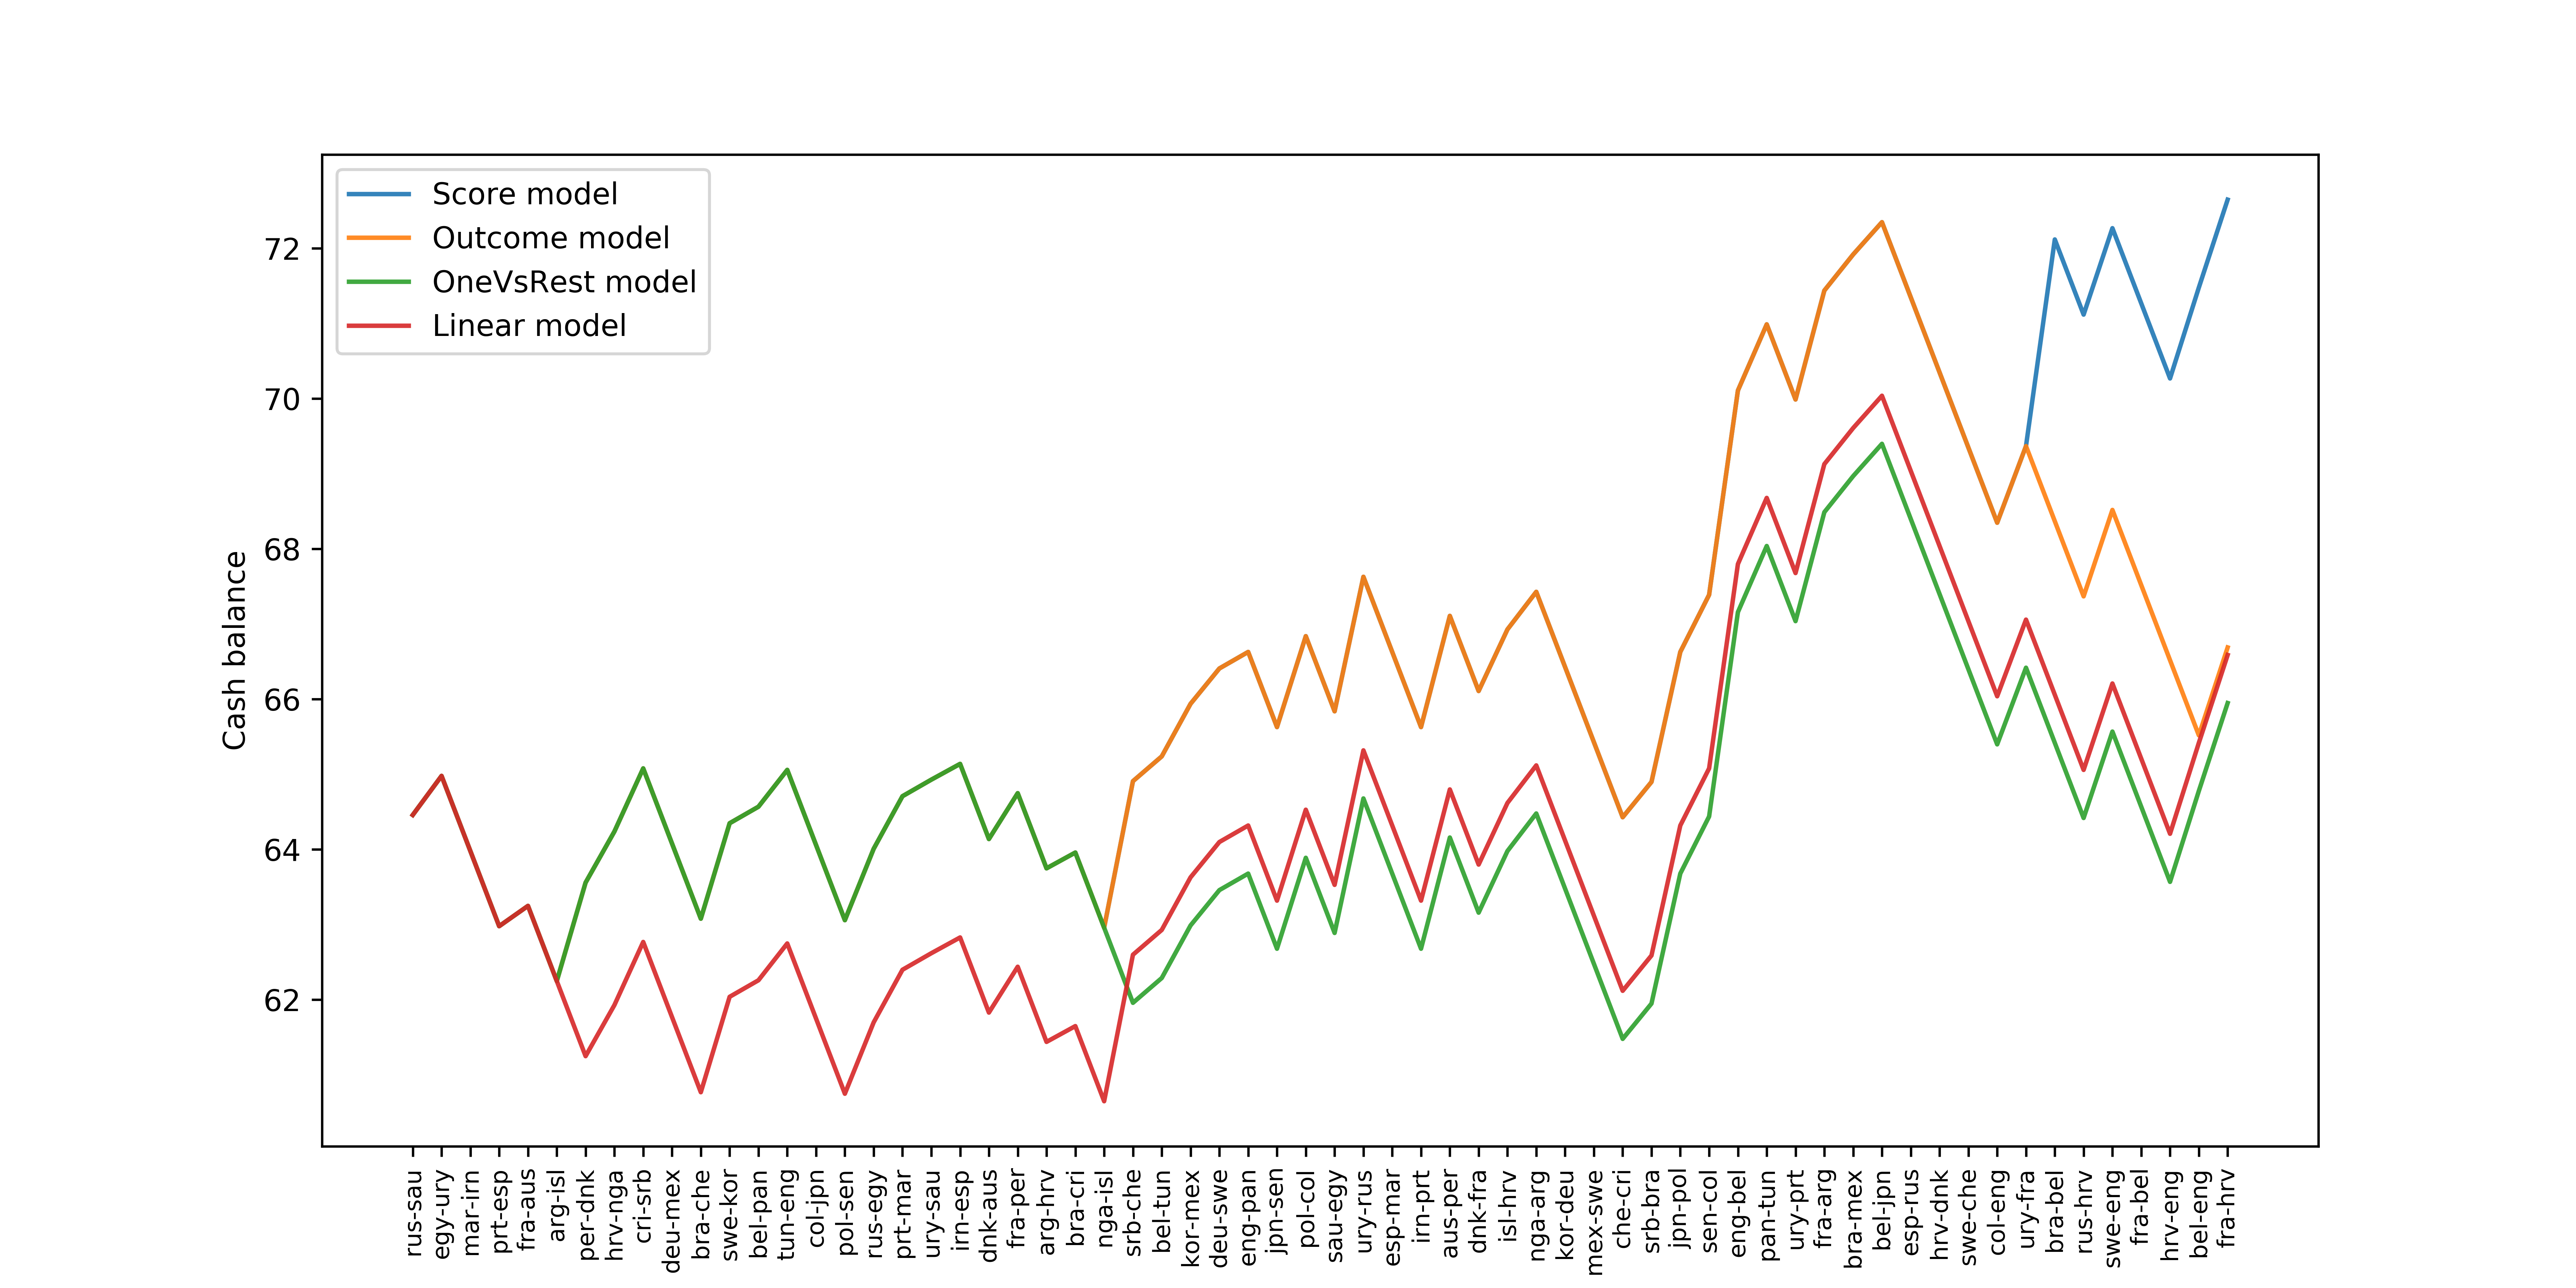
\includegraphics[width=1\textwidth]{img/match_level_2018_model_unit.png}
    \caption{Unit strategy's cash balance progression on World Cup 2018.}
    \label{fig:unit_model_comparison}
\end{figure}

\begin{figure}[H]
    \centering
    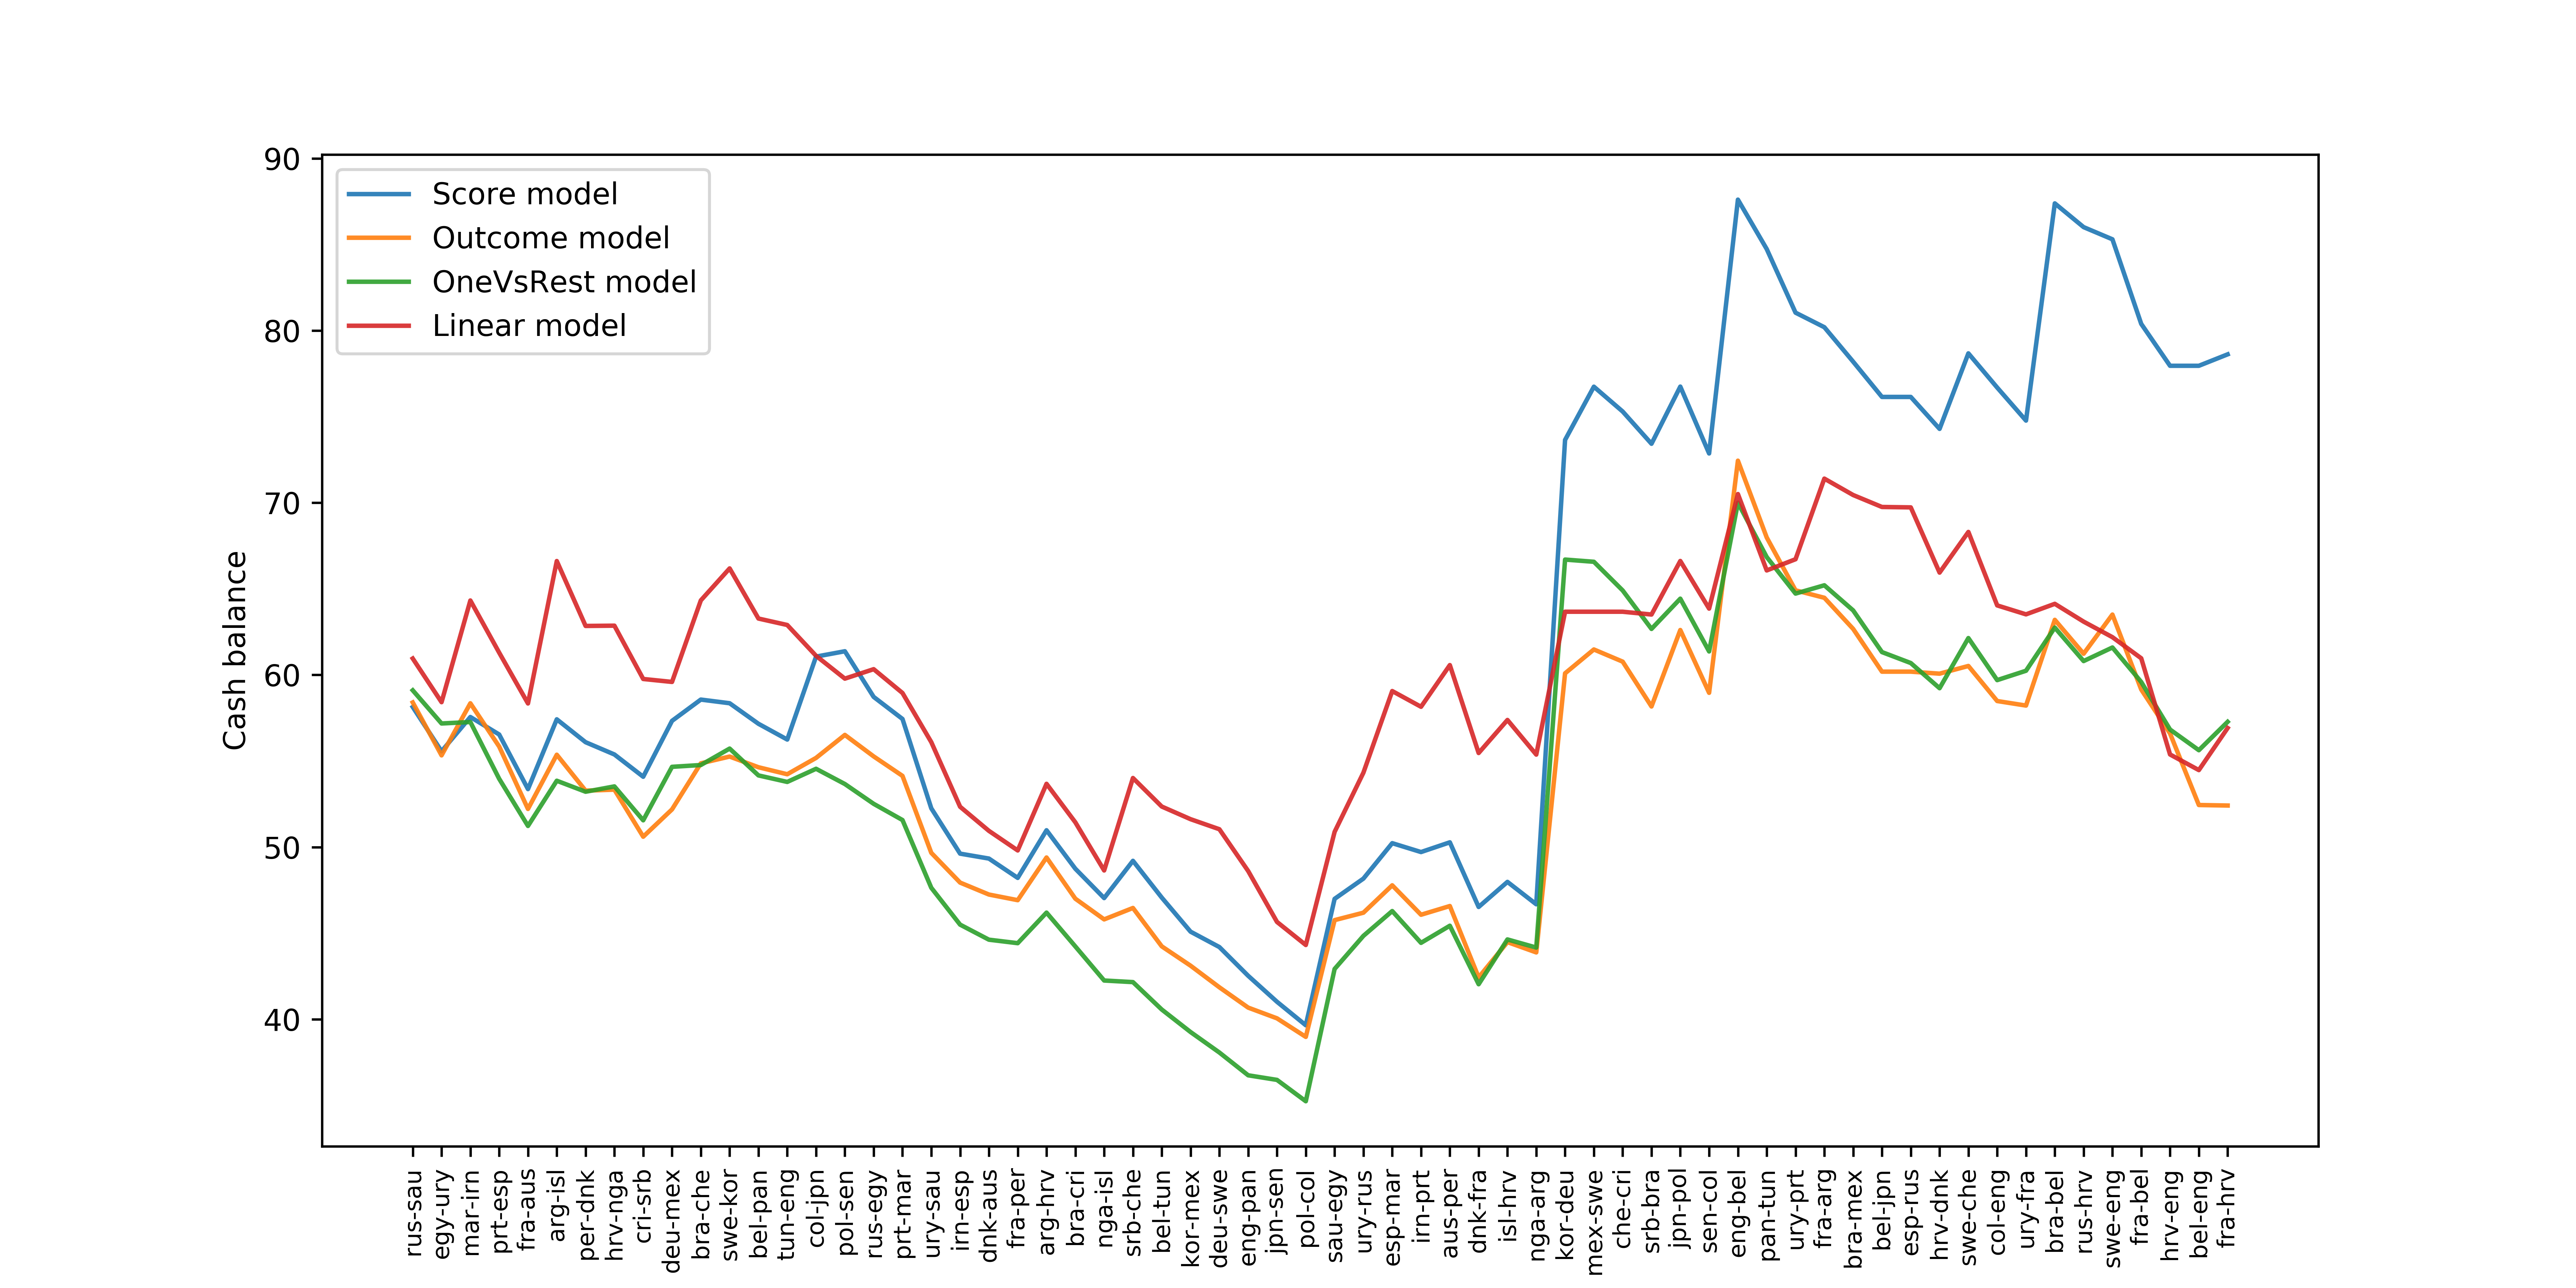
\includegraphics[width=1\textwidth]{img/match_level_2018_model_kelly.png}
    \caption{Kelly strategy's cash balance progression on World Cup 2018.}
    \label{fig:kelly_model_comparison}
\end{figure}

\begin{figure}[H]
    \centering
    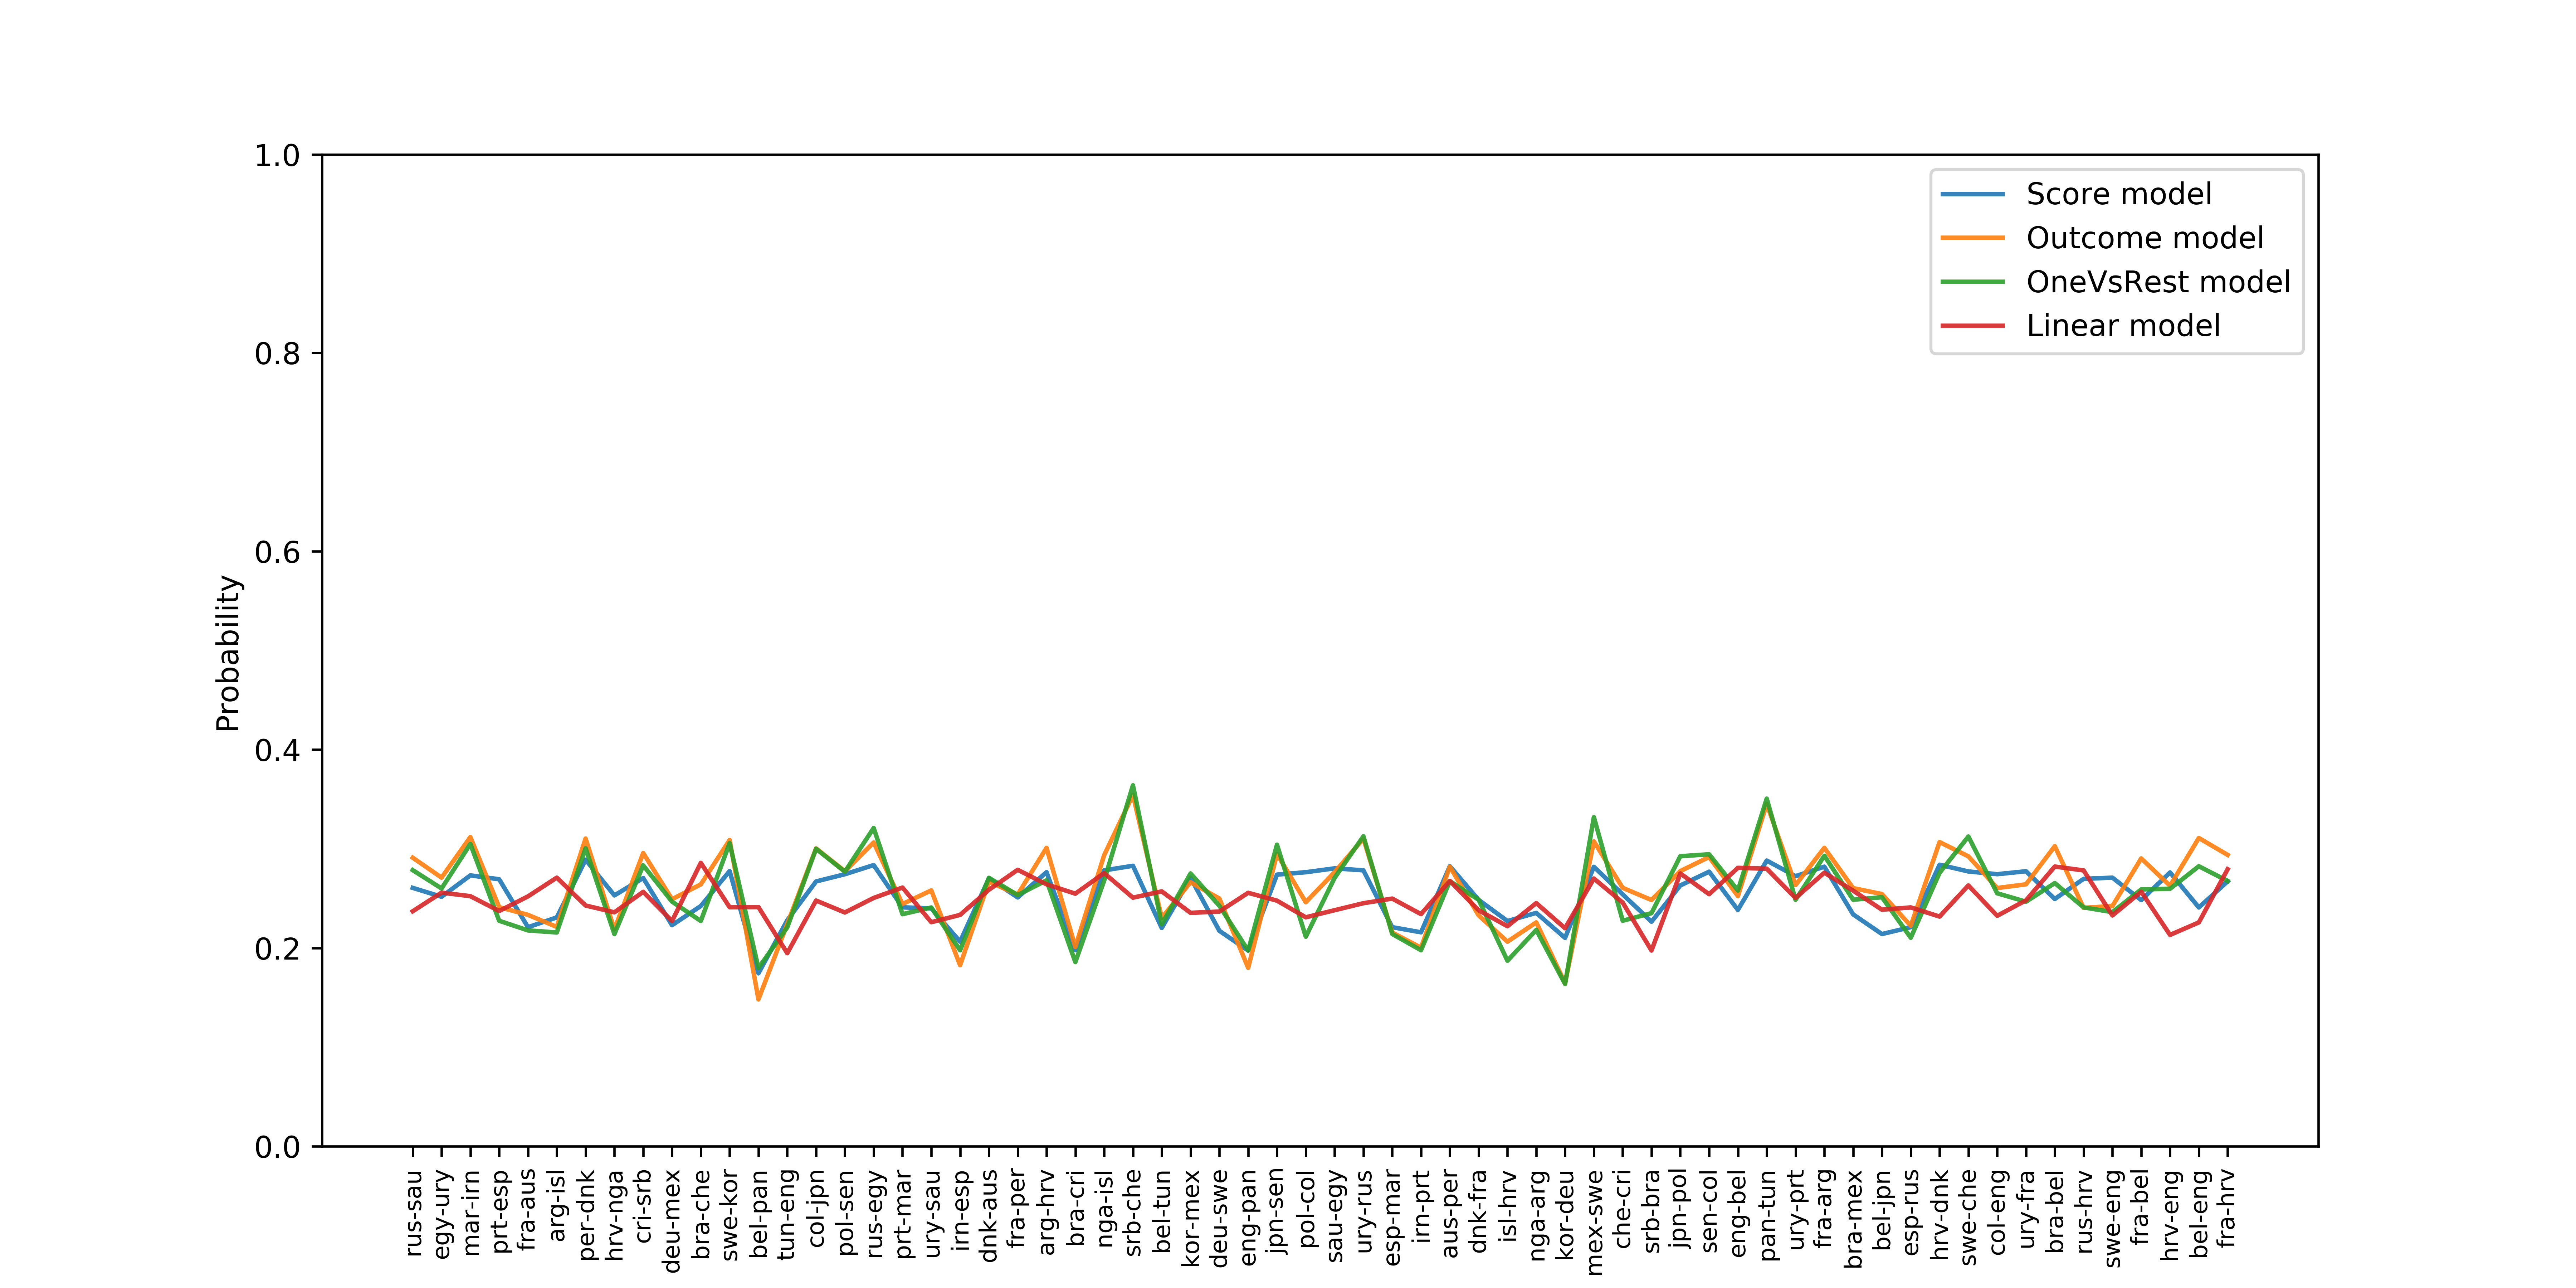
\includegraphics[width=1\textwidth]{img/match_level_2018_model_probability_draw_prob.png}
    \caption{Predicted probability of draw in the World Cup 2018.}
    \label{fig:draw_probability}
\end{figure}

\begin{figure}[H]
    \centering
    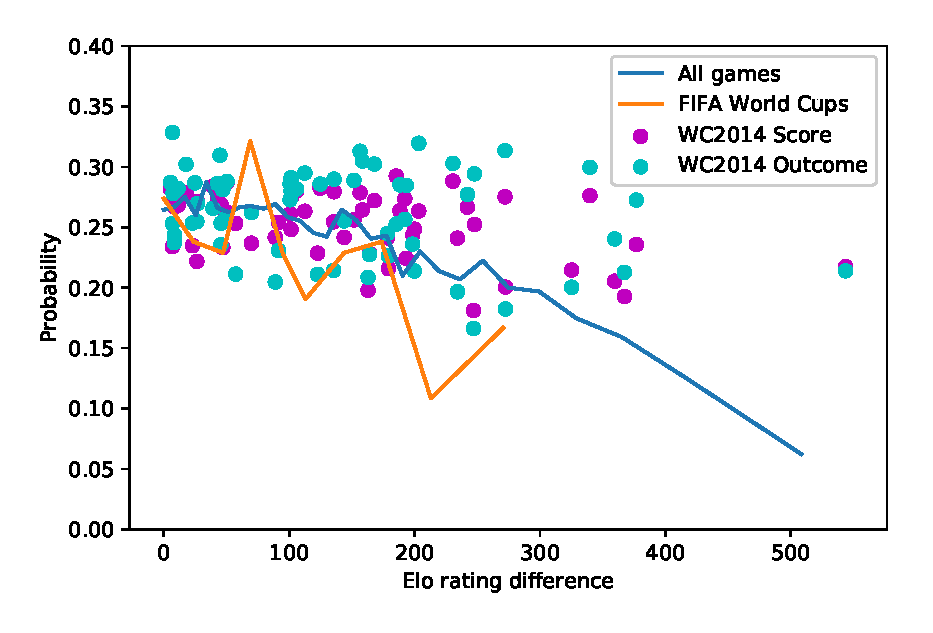
\includegraphics[width=1\textwidth]{img/draw_true_probability_wc.eps}
    \caption{Predicted probabilities vs. sample probability distribution. Sample probability distribution of draw is calculated from all international football games between dates 11/30/1872 - 06/04/2018. Dots are single probability estimates from \textit{Score model} and \textit{Outcome model} for matches in World Cup 2014.}
    \label{fig:draw_prob_dist}
\end{figure}

\section{Feature set comparison}
It's interesting that feature sets with fewer features can produce better predictions. How can less describe more? It's against common sense, right?

These problems are visible if the models' accuracy is compared. Being one of the most important metrics, it's still not the most important for the sophisticated betting strategies like kelly, which utilizes model's probability estimates. Log loss is a metric that can be used to compare probability distributions' accuracy. A smaller value indicates a more accurate estimate. When log loss is compared per tournament model trained with limited feature set can have lower log loss value than the same model that is trained using all of the features. But when the average performance from every tournament is considered training model with all features seems to output the lowest log loss score with \textit{Outcome model} and \textit{OVR model} and second lowest (only 0.0009 difference at highest) with \textit{Score model} and \textit{Linear model}. This indicates that even-though increasing accuracy might not benefit from using all features probability distribution prediction clearly benefits. Since football games often have low scores can last-minute surprises change the outcome of the match. The underdog can beat the favorite or at least square the game. This means that achieving high accuracy is hard, but fixing probabilities to match the true ones has more room to improve.

Feature importance can be calculated with Random Forest. These values can give insight on models reasoning. This data combined with optimal hyperparameters is one way to interpret the models since inspecting every single tree in the forest would be too cumbersome.

Segal \cite{segal2004machine} showed that noisy variable can lead to higher optimal value for minimum samples at leaf hyperparameter. With generic features models seem to prefer higher value for the hyperparameter \textit{minimum samples at leaf} as we can see from the table \ref{table:hyperparam_results}.  Figure \ref{fig:outcome_feature_importance_gf} lists feature importance for Outcome model trained with generic features. Difference between elo rating dominates the others, but just by looking at the plot it's impossible to say if any of the features could be considered to be just noise. Lower importance features like \textit{home\_goal} and \textit{away\_goal} seem to be in the middle tier when model is trained with all features. This higher importance compared to other features could mean that these features have predicting power.

With \textit{player features} difference between features is not that big. Feature importance is gradually decreasing feature by feature as we can see from the figure \ref{fig:outcome_feature_importance_pf}. Same features seem to rank high with player features as they would with all features.

\begin{table}
    \caption{Hyperparameter selection results for random forest models.}
    \begin{tabular}{| c  c| c| c| c|}
        \hline
        Model & Features & \# of predictors & Min samples at leaf & Max depth\\
        \hline
        Score & AF & $\sqrt{M}$ & 1 & 8 \\
         & GF & $\log_2{M}$ & 10 & 8 \\
         & PF & $\sqrt{M}$ & 5 & Na \\
         \hline
        Outcome & AF & $\sqrt{M}$ & 3 & 8 \\
         & GF & $\log_2{M}$ & 15 & 5 \\
         & PF & $\log_2{M}$ & 3 & 8 \\
        \hline
        OVR & AF home win & $\sqrt{M}$ & 3 & 5 \\
        OVR & AF draw & $\sqrt{M}$ & 5 & Na \\
        OVR & AF away win & $\sqrt{M}$ & 3 & 5 \\
        OVR & GF home win & $\sqrt{M}$ & 10 & 12 \\
        OVR & GF draw & $\log_2{M}$ & 15 & 8 \\
        OVR & GF away win & $\log_2{M}$ & 10 & 5 \\
        OVR & PF home win & $\log_2{M}$ & 3 & 5 \\
        OVR & PF draw & $\log_2{M}$ & 15 & 5 \\
        OVR & PF away win & $\log_2{M}$ & 5 & 8 \\
        \hline
    \end{tabular}
    \label{table:hyperparam_results}
\end{table}

\begin{figure}[H]
    \centering
    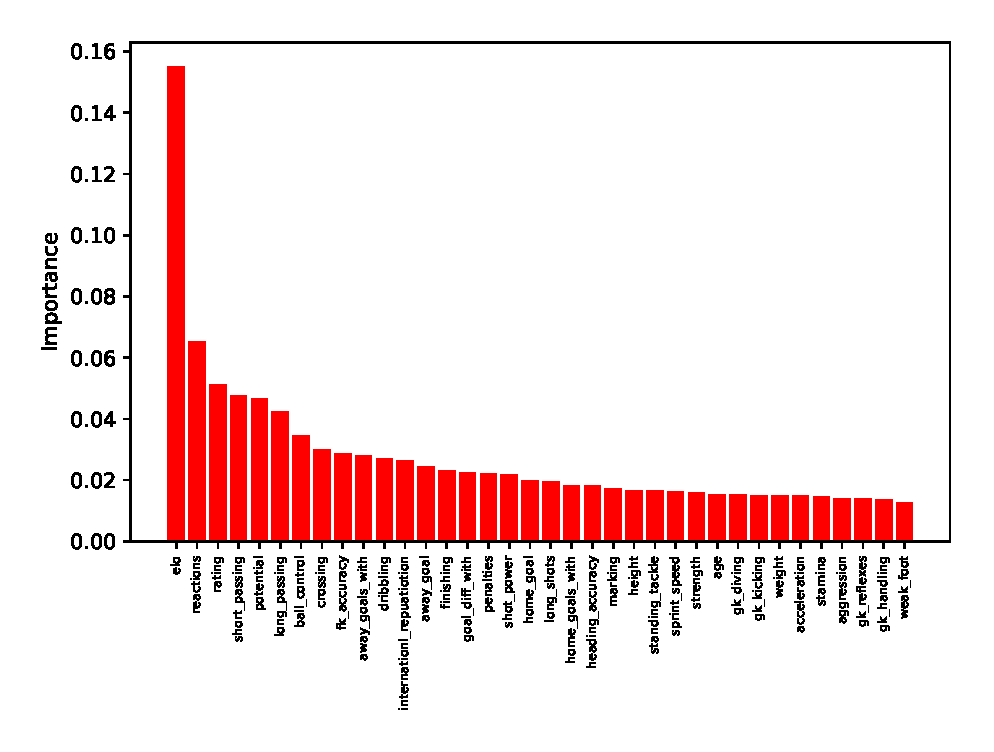
\includegraphics[width=1\textwidth]{img/match_level_2018_outcome_feature_importance_af_feature_importance.eps}
    \caption{Outcome model's feature importance with all features.}
    \label{fig:outcome_feature_importance_af}
\end{figure}

\begin{figure}[H]
    \centering
    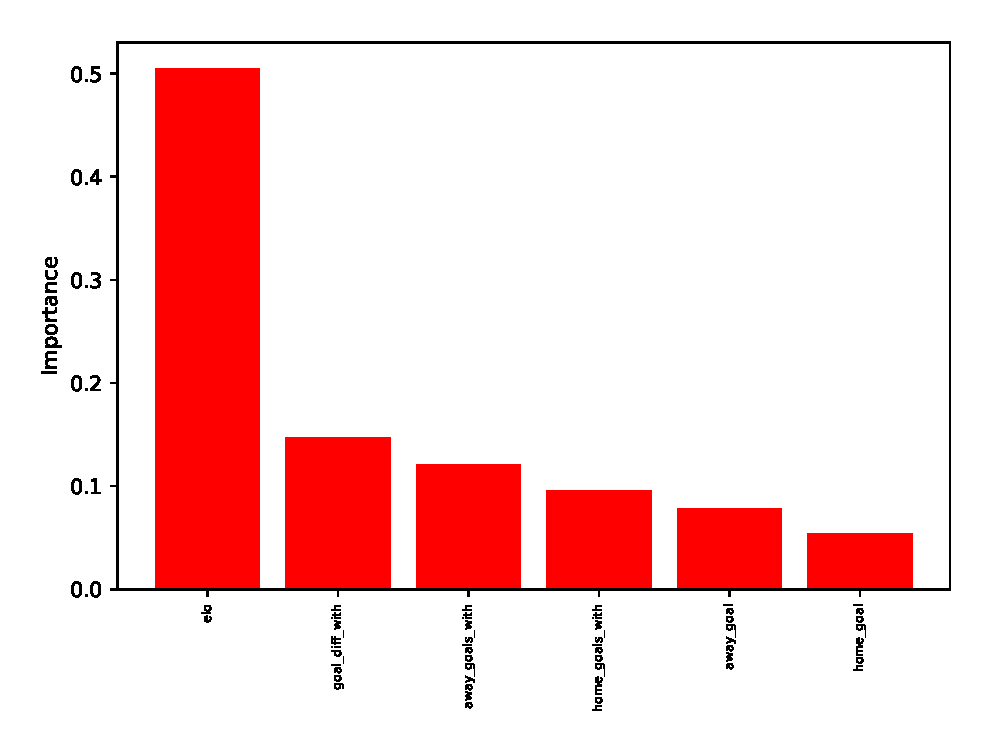
\includegraphics[width=1\textwidth]{img/match_level_2018_outcome_feature_importance_gf_feature_importance.eps}
    \caption{Outcome model's feature importance with generic features.}
    \label{fig:outcome_feature_importance_gf}
\end{figure}

\begin{figure}[H]
    \centering
    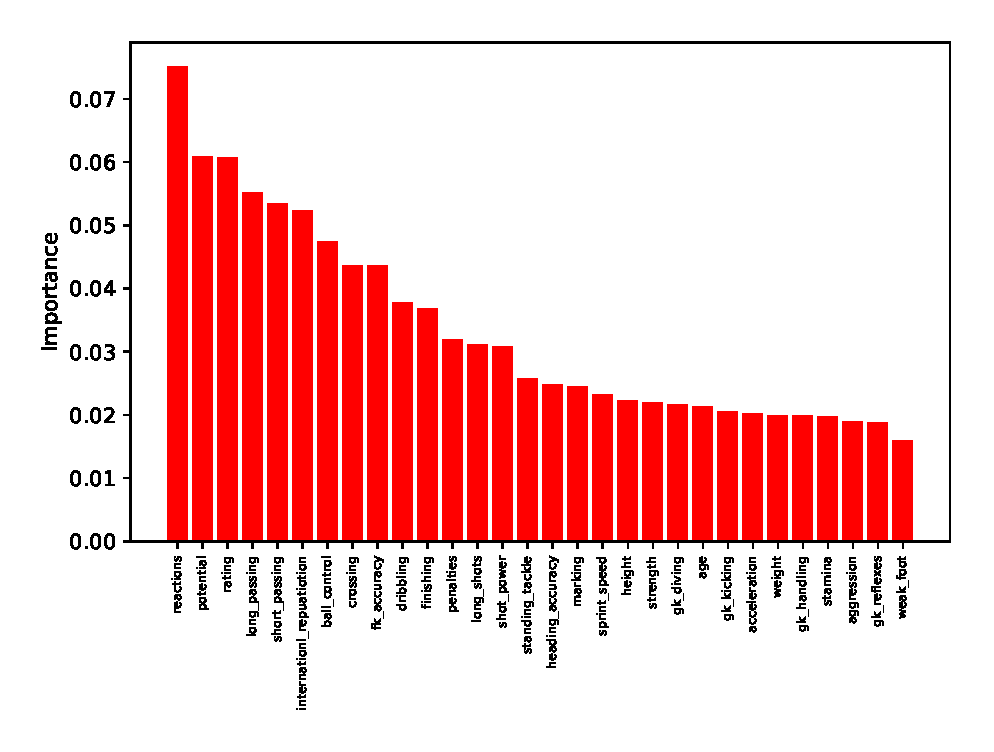
\includegraphics[width=1\textwidth]{img/match_level_2018_outcome_feature_importance_pf_feature_importance.eps}
    \caption{Outcome model's feature importance with player features.}
    \label{fig:outcome_feature_importance_pf}
\end{figure}

If some of the features are just noise, those features can be removed without harming the model's probability estimates. One way to do this is recursive feature elimination where one by one features are eliminated and models performance is measured for every elimination round. This test is done 100 times for every elimination round to guarantee that variation in the results won't cause features to be eliminated too early. I did the recursive feature elimination process the \textit{Outcome model}.

\section{Recursive feature elimination}
If some of the features are just noise, those features can be removed without harming the model's probability estimates. One way to do this is recursive feature elimination (RFE) where one by one features are eliminated and models performance is measured for every elimination round. The least important feature is eliminated each round. Accuracy and log loss are measured 100 times for each round to account for natural variance in the results. Feature elimination process is started again until there are no features left. Stored average accuracy and average log loss can be used to see how the model's performance evolved during RFE. All of the test were done with \textit{Outcome model}.

First test included default parameters for \textit{Outcome model}: 1000 for number of estimators, $\sqrt{M}$ for number of predictors, Na for maximum depth and one for minimum samples at leaf. From figure \ref{fig:def_avg_accu} we can see that after \textit{gk\_diving} accuracy starts to decrease slowly. If we compare this result to figure \ref{fig:def_avg_loss}
it's evident that the performance decreases after \textit{gk\_diving}. For comparison I run the same test with \textit{Outcome model} using optimal parameters used in all feature setup in the table \ref{table:outcomemodel}. Results are visible in the figures \ref{fig:optimal_avg_accu} and \ref{fig:optimal_avg_loss}. With this setup model performs better through out the whole RFE process. Also, model peaks the highest accuracy with only just four features. Improvement with this same feature set is not visible in the average log loss. The average log loss has a clear performance drop only when there is a single feature left.

To test model's performance with limited feature set I ran the World cup simulation for \textit{Outcome model} using features: \textit{away\_goals\_with\_home, finishing\_diff, height\_diff, crossing\_diff, potential\_diff, fk\_accuracy\_diff, home\_goal\_mean, away\_goal\_mean, ball\_control\_diff, long\_passing\_diff,  short\_passing\_diff, reactions\_diff, rating\_diff, elo\_diff}. I chose these features since they were the smallest feature set that was able to keep the performance with a model trained with default hyperparamaters. New optimal hyperparameters where grid searched for this feature set. These hyperparameters are listed in the table \ref{table:hyperparam_results_rfe} and World Cup simulation results are in the table \ref{table:outcomemodel_rfe}. Based on the results model's performance according to accuracy and log loss doesn't differ significantly from the model that was trained using all features.

Based on the progression of the average accuracy and the average log loss models do not perform better when features are removed from the original feature set. Eventually performance decreases but never increases during feature elimination. Most of the time results just have natural variance, which causes small changes. It seems that using every available feature doesn't harm random forest's performance, even though there is no guarantee that all of the features are useful. Also, RFE's suitability for this setup can be questioned. Stroble et al. concluded: "In particular, the selection of the first splitting variable involves only the marginal, univariate association between that predictor variable and the response, regardless of all other predictor variables. However, this search strategy leads to a variable selection pattern where a predictor variable that is per se only weakly or not at all associated with the response, but is highly correlated with another influential predictor variable, may appear equally well suited for splitting as the truly influential predictor variable." This can be problematic since removing one of the correlated predictors decreases impurity significantly and this effect is not as visible when the rest of the correlated predictors are removed. This leads to a situation where importance of a feature is measured incorrectly.
\begin{figure}[H]
    \centering
    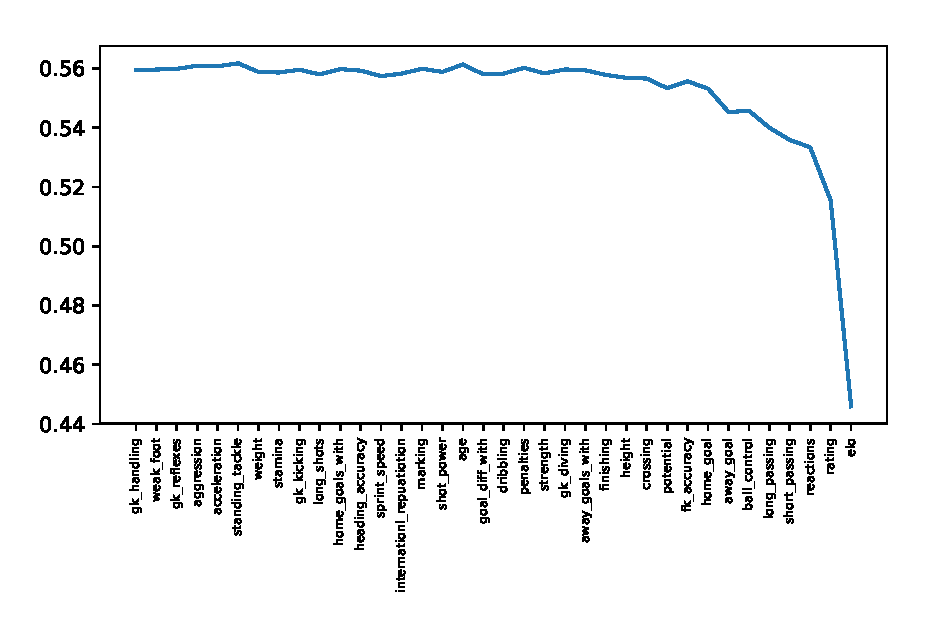
\includegraphics[width=1\textwidth]{img/default_avg_accuracy.eps}
    \caption{Mean accuracy for recursive feature elimination on outcome model with default parameters.}
    \label{fig:def_avg_accu}
\end{figure}

\begin{figure}[H]
    \centering
    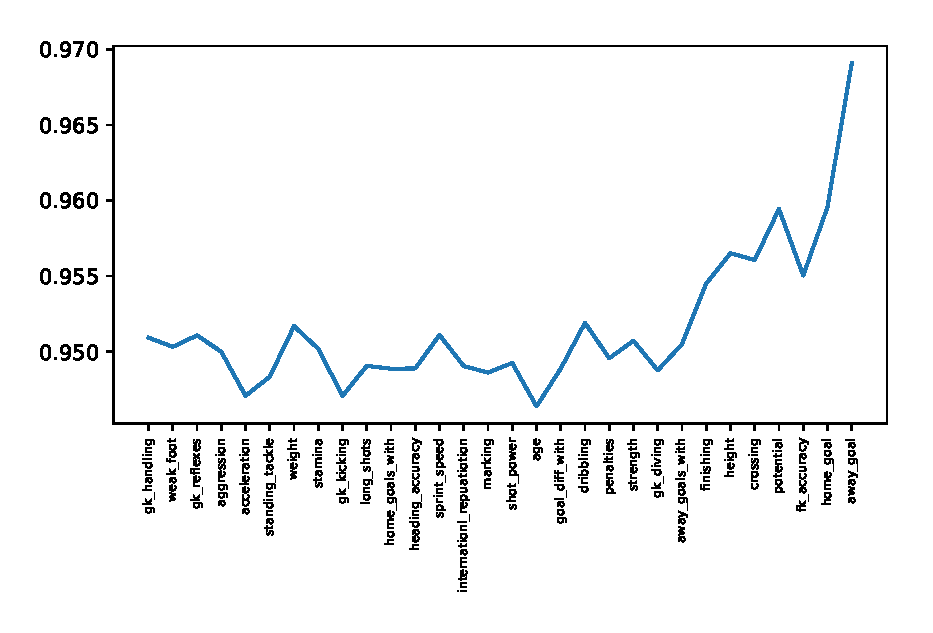
\includegraphics[width=1\textwidth]{img/default_avg_lloss.eps}
    \caption{Mean log loss for recursive feature elimination on outcome model with default parameters. Only features from first round to the 30th round are list to ensure figure's readability.}
    \label{fig:def_avg_loss}
\end{figure}

\begin{figure}[H]
    \centering
    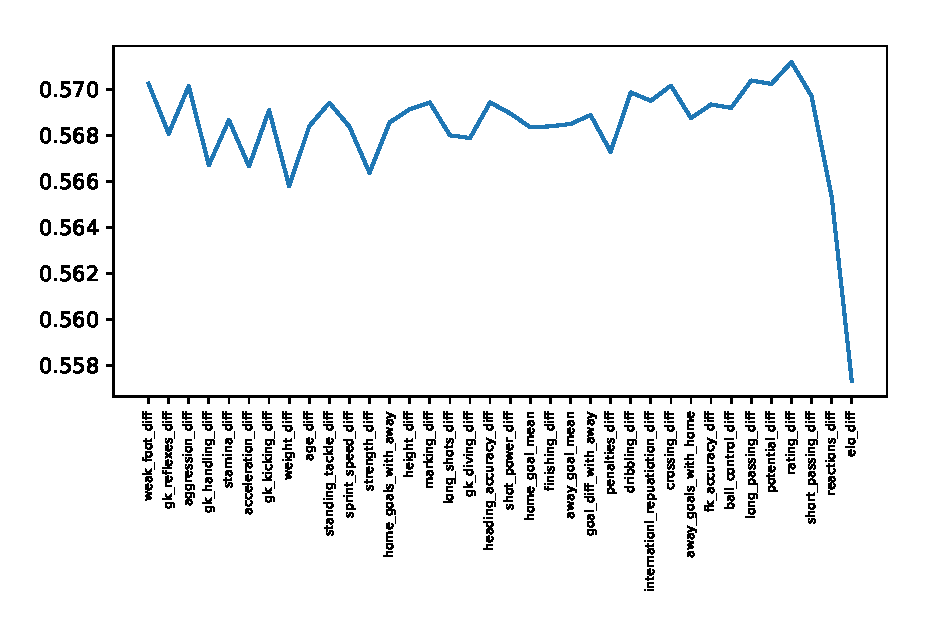
\includegraphics[width=1\textwidth]{img/optimal_avg_accuracy.eps}
    \caption{Mean accuracy for recursive feature elimination on outcome model with optimal parameters for all features setup in the table \ref{table:outcomemodel}.}
    \label{fig:optimal_avg_accu}
\end{figure}

\begin{figure}[H]
    \centering
    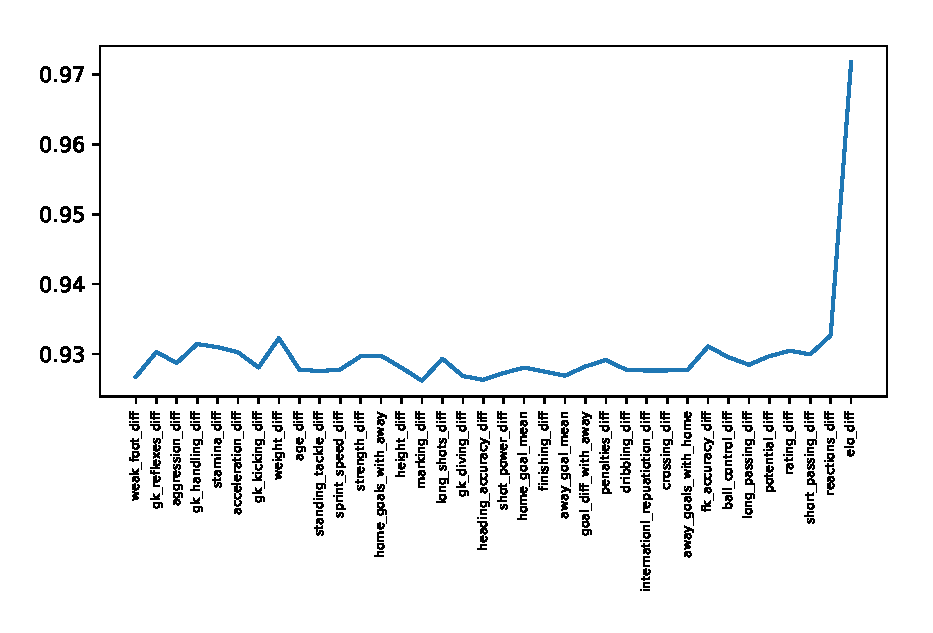
\includegraphics[width=1\textwidth]{img/optimal_avg_lloss.eps}
    \caption{Mean log loss for recursive feature elimination on outcome model with optimal parameters for all features setup in the table \ref{table:outcomemodel}.}
    \label{fig:optimal_avg_loss}
\end{figure}

\begin{table}
    \caption{Results for Outcome model with limited features from RFE.}
    \begin{tabular}{| c | c| c| c|c|}
        \hline
        Metric& \textbf{WC 2018} & \textbf{WC 2014} & \textbf{WC 2010} & Mean\\
        \hline
        Accuracy  & 52.97\% $\pm$ 2.36 & 59.69\% $\pm$ 2.3 & 56.09\% $\pm$ 2.47& 56.25 \\
        Log Loss & 0.9953 $\pm$ 0.0087 & 0.9282 $\pm$ 0.0061 & 0.9743 $\pm$ 0.0069& 0.9659 \\
        Unit profit  & -1.79\% $\pm$ 6.16 & 14.12\% $\pm$ 6.02 & 8.82\% $\pm$ 7.47& 7.05 \\
        Kelly profit  & -37.19\% $\pm$ 11.43 & 61.45\% $\pm$ 15.42 & 77.87\% $\pm$ 12.98& 34.04 \\
 \hline
    \end{tabular}
    \label{table:outcomemodel_rfe}
\end{table}

\begin{table}
    \caption{Optimal hyperparameters for Outcome model trained with RFE feature set.}
    \begin{tabular}{| c | c| c| c|}
        \hline
         \# of predictors & Min samples at leaf & Max depth\\
        \hline
         $\sqrt{M}$ & 10 & Na \\
        \hline
    \end{tabular}
    \label{table:hyperparam_results_rfe}
\end{table}


\section{Match-level betting activity - what drives the profits?}
As it's mentioned many times unit strategy can be considered as a dummy strategy; one unit for the predicted winner. Kelly strategy instead is more sophisticated and deserves a deeper analysis. With the requirements 1) profitable in every tournament, and 2) best average profits has \textit{Score model} trained with all features performed the best with kelly strategy. For this reason \textit{Score model} is used to get the results for the following figures.

The most successful tournament for \textit{Score model} was World Cup 2018. It achieved, on average, 35.59\% profit. In comparison profit from World Cup 2014 was only 12.37\%. By the numbers performance in World Cup 2018 was definitely better, but what happened with match-level betting? When we compare both of the tournaments side by side in the figures \ref{fig:net_win_cost_2018} and \ref{fig:net_win_cost_2014} it's clear that a single successful bet dominates the profit in World Cup 2018. Don't get confused by the difference in the scale of y-axis. Total bets per match are not that different between the tournaments. Only betting frequency differs - there are more games in World Cup 2014 without any bets. With World Cup 2018 winnings are more rare, but the size is bigger. These anomalies in odds are certainly important and this strategy is able to utilize them properly. Without three biggest winnings this strategy would achieve negative profits for sure. With World Cup 2014 strategy wins more often, but winning as not as big as they are in World Cup 2018. This would be ideal as well for the World Cup 2018, but it's harder to achieve. When winnings are more frequent predicted probabilities need to be closer to the true ones than the implied probabilities from the betting market are. Based on the limited amount of evidence, smaller but more frequent winnings and sparser betting activity, it seems that the probability estimates for World Cup 2014 were better than the implied ones based on the market. Where as in World Cup 2018 profitability was based on the strategy's ability to gain from few favourable odds. The latter might be extremely hard to keep profitable in the long run unless betting market's dynamics create opportunities often enough. Model's bias towards higher probability of a draw compared to market's when difference between teams' elo rating is relatively high stands out in both of the tournaments. This harms the strategy's performance.

\begin{figure}[H]
    \centering
    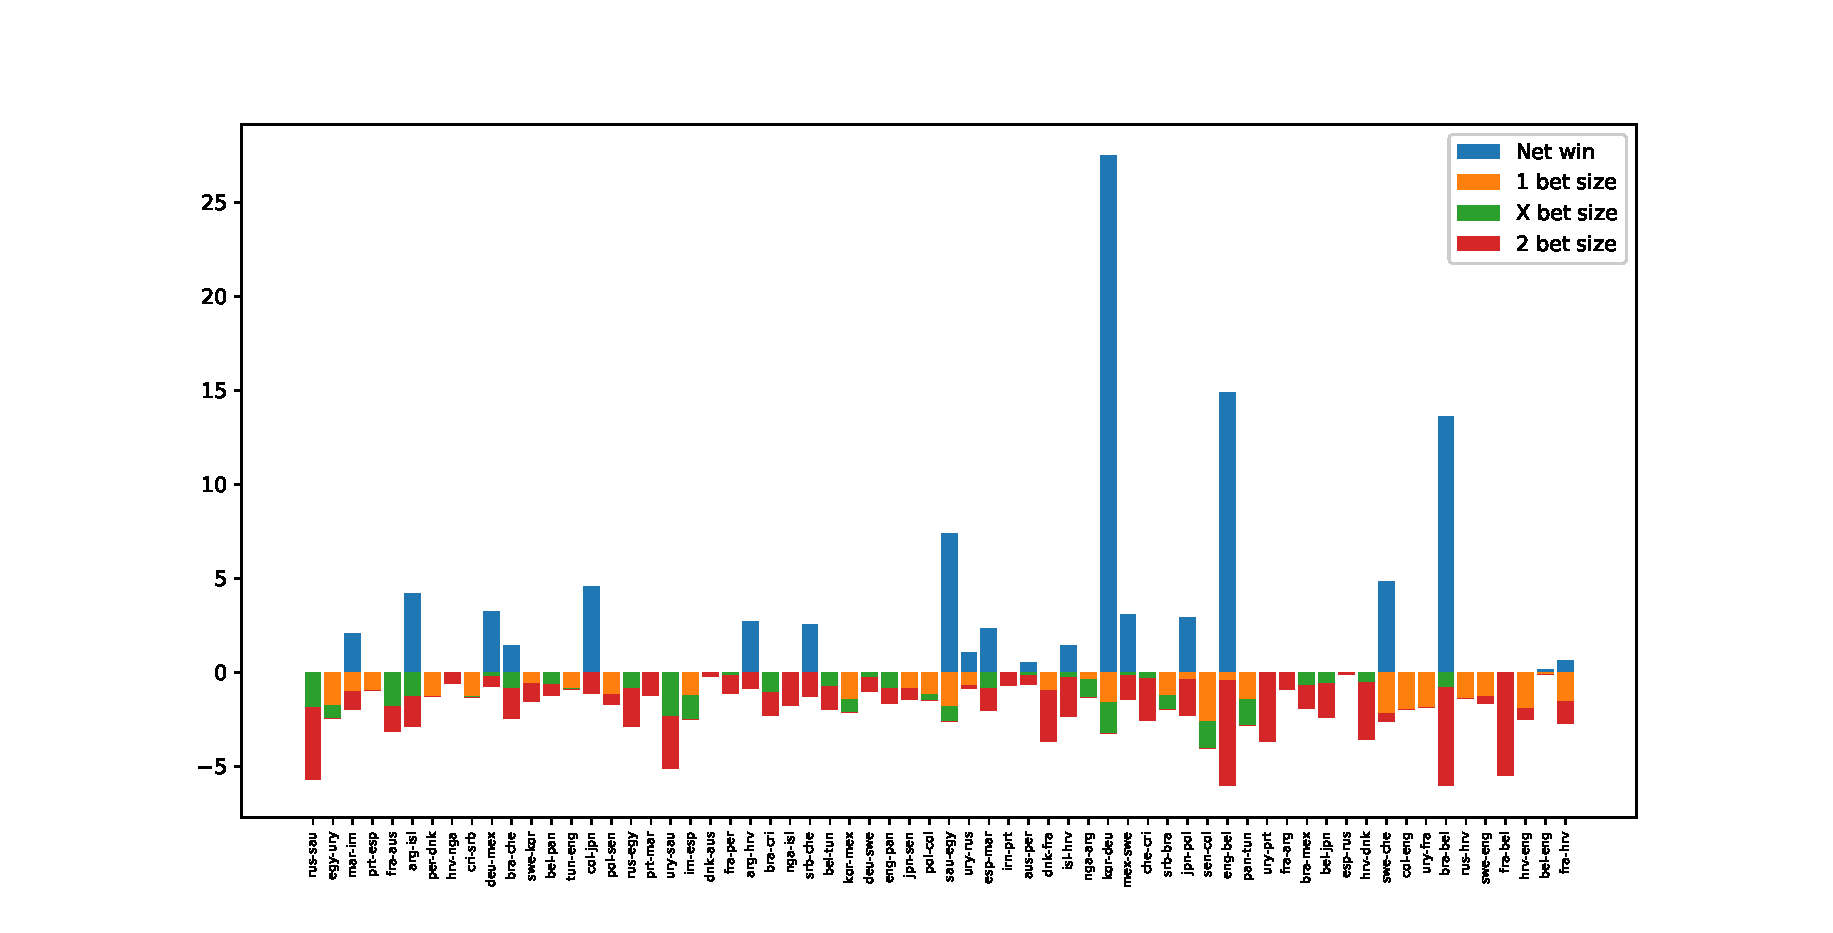
\includegraphics[width=1\textwidth]{img/match_level_2018_score_win_cost_.eps}
    \caption{Net winnings and betting costs per label for Score model in World Cup 2018.}
    \label{fig:net_win_cost_2018}
\end{figure}

\begin{figure}[H]
    \centering
    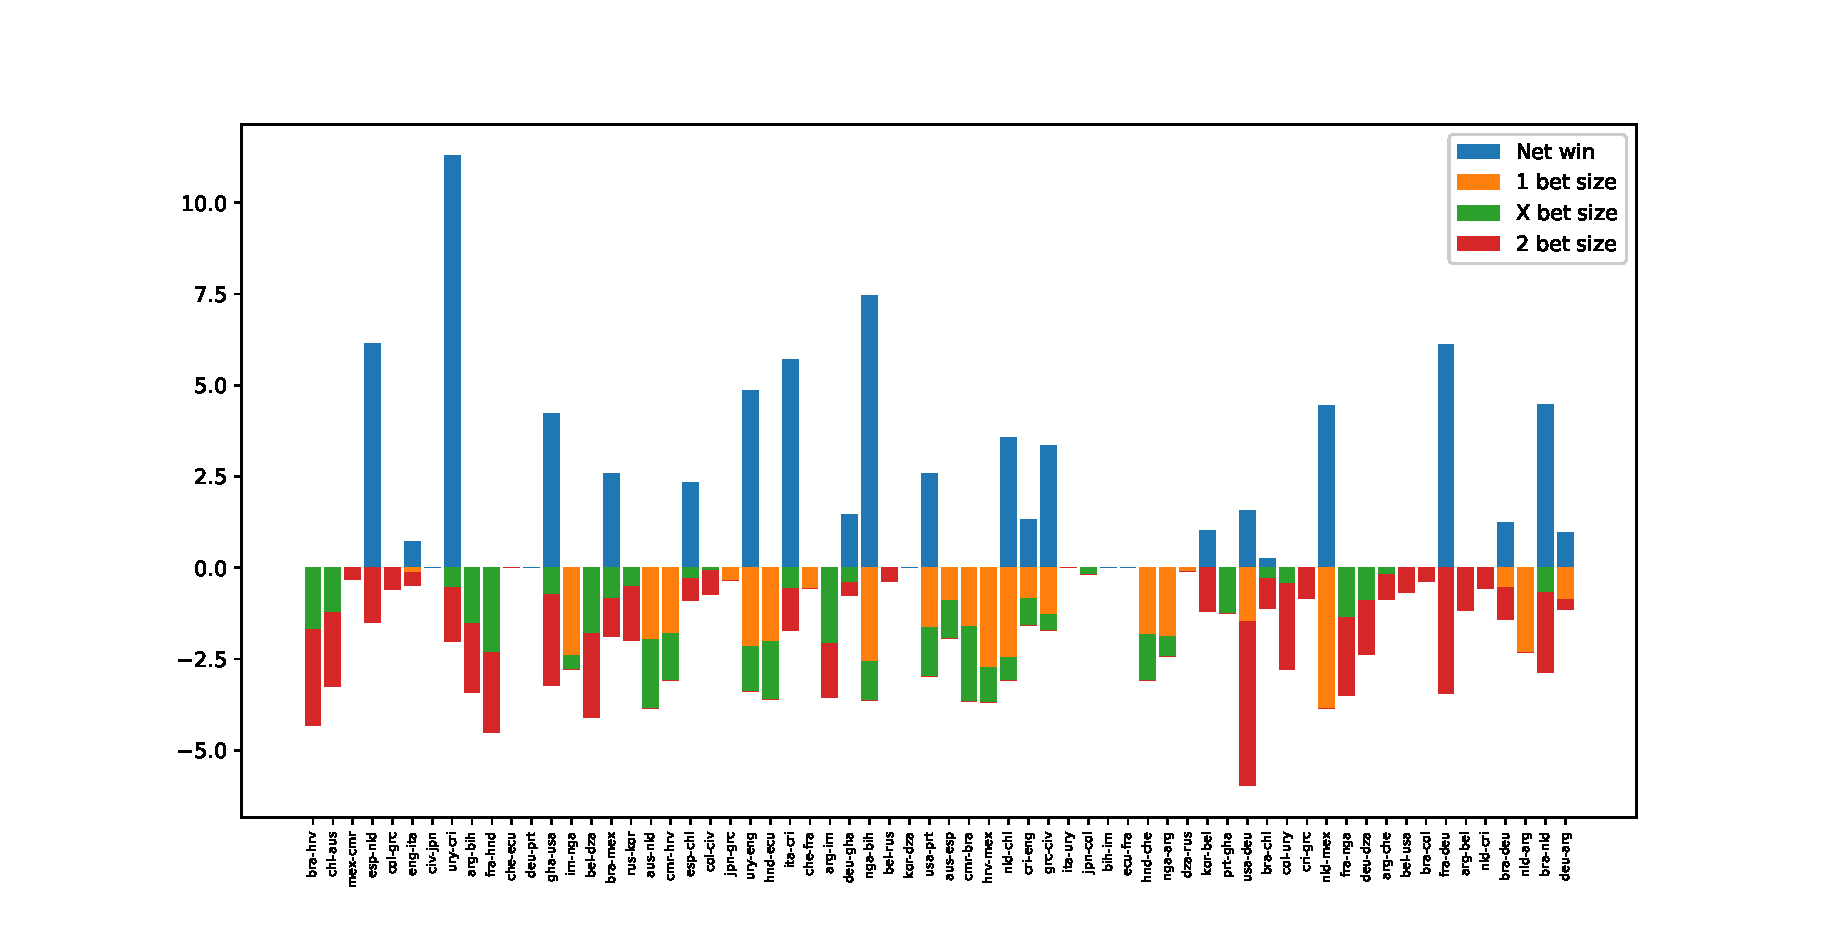
\includegraphics[width=1\textwidth]{img/match_level_2014_score_win_cost_.eps}
    \caption{Net winnings and betting costs per label for Score model trained with all features in World Cup 2014.}
    \label{fig:net_win_cost_2014}
\end{figure}

\chapter{Conclusion}
In this thesis, I have investigated the possibility to "beat the bookie" on FIFA World Cup. To achieve this the profits from betting need to be positive and the models should have better prediction accuracy than the bookmaker has. In my experiments, I have used four different models with three different combinations of features. For betting two different strategies were used. All the data used in the experiments was freely available on the internet.

Reference model, the bookmaker's model, was formed using the average odds provided for the match. This model achieved the accuracy of 56.25\% for World Cup 2018 and 2014, and 51.56\% for World Cup 2010. In total, 28 out of the all 36 model and feature set combinations were able to beat the bookmaker's model in prediction accuracy. "Beating the bookie" in prediction accuracy is doable.

Being profitable with both of the betting strategies in all of the tested World Cup tournaments: 2018, 2014, and 2010 is possible. More importantly, it's possible to earn on average as high as 24.05\% returns using Kelly strategy. The other strategy, unit strategy, has less variance but the fixed bet size limits its ability to maximize the profits from abnormal odds. Unit strategy's returns are more often positive, but lower in size. The answer to the question
"Is it possible to 'beat the bookie'?" is \textit{yes}. However, this result should be approached with caution. Combined results from three World Cups contains only 192 games, which means that the sample is small. It would be ideal to test this with more tournaments if data would be available. Football leagues have more games and one option to do further validation on this would be to simulate for example one season of English Premier League (EPL). Also, the lag of 4 years between the tournaments gives bookmakers plenty of time to improve their models. Already results from the latest World Cup indicate that good opportunities exist more rarely; profits are more connected to few games and only 7 out of 12 of the models were able to outperform the reference model's accuracy. There are no guarantees that the profits from the upcoming World Cup 2022 will be positive.

Extensive feature analysis with tree-based models indicates that no subset of features gives better results than using all of the features. Some of the tournament simulation results are in contrary to this since in some cases using a limited feature set improves the result of a single tournament simulation. However, when all tournaments are considered using all of the features seems to be the best option. Instead of further optimizing the perfect feature set the features themselves should be investigated. Maybe the current way of aggregate the team-level features could be improved to really differentiate the teams. Also, more data, like lineups, could be included to improve the feature's accuracy. Using optimal hyperparameters turned out to be an important way to improve the results. When recursive feature elimination was performed for the  \textit{Outcome model} using the default hyperparameters and the optimal hyperparameters for all features setup the model that used optimized hyperparameters performed better throughout the RFE. The grid search strategy for finding the optimal hyperparameters was successful.

Predicting draws turned out to be really demanding. What could be done to improve this? This thesis will not provide a clear answer. Models predicted draws differently but no model was clearly better than the rest. The reference model was no better in accuracy. Improving the prediction accuracy of a draw would be most likely very beneficial and hopefully initiates further research.



\bibliography{references.bib}
\bibliographystyle{IEEEtran}

\end{document}